\documentclass[a4paper,11pt]{article}
\usepackage[style=ieee,backend=bibtex]{biblatex} 
\usepackage{amsmath,amsfonts}
\usepackage{geometry}
\usepackage{bm}
\usepackage{longtable} % for 'longtable' environment
\usepackage{pdflscape} % for 'landscape' environment
\usepackage{rotating}
\usepackage{tabularx}
\usepackage{multirow}
\usepackage[binary-units]{siunitx}
\usepackage{pgfgantt}
\usepackage{float}
\usepackage{svg}
\usepackage{hyperref}
\usepackage[version=4]{mhchem}

\bibliography{main.bib,websites.bib,datasheets.bib} % TODO: MAKE ACCESSED BY note PARAM AND SHIT NORMAL BETWEEN ALL REFERENCES.

% Declare custom (Non-si) units
\DeclareSIUnit\feet{ft} % Yes I know feet aren't SI unit...
\DeclareSIUnit\year{y}
\DeclareSIUnit\gacc{\textit{g}}
\DeclareSIUnit\siaxis{\text{axis}}
\DeclareSIUnit\baud{bd}
\DeclareSIUnit\mmDA{mm\, DA}
\DeclareSIUnit\octave{oct}

% https://tex.stackexchange.com/a/121871
\newcommand*{\fullref}[1]{\hyperref[{#1}]{\ref*{#1} \nameref*{#1}}}

\newcommand{\liion}{\ce{Li}-ion}

\ganttset{calendar week text={\small{\startday/\startmonth}}}

\begin{document}


\begin{titlepage}

% Center the content
\begin{center}

% Title
% \vspace*{3cm}
% ATTENTION: THIS IS A DRAFT VERSION. TODO: CHECK GRAMMAR AND PRESENTATION BEFORE SUBMITTING
{\LARGE\bfseries Design of an Experiment to Evaluate High-Power Rockets as a CubeSat Qualification Platform} \\[3cm]



% Author's name
{\Large Author: Peter Tanner} \\[1cm]

% Supervisor's name
{\Large Supervisor: Dilusha Silva} \\[2cm] % \\[3cm]

% Degree text
{\large ATTENTION: THIS IS A DRAFT VERSION. TODO: CHECK GRAMMAR AND PRESENTATION BEFORE SUBMITTING}
{\large \textit{This thesis is presented in partial fulfilment of the requirements for the degree of Bachelor of Philosophy
(Honours) at the University of Western Australia}} \\[1cm]

% Faculty information
{\large Faculty of Engineering and Mathematical Sciences} \\[3cm]

{\large Word count: TODO:} \\
{\large Submitted: \today} \\[2cm]

\includesvg[width=0.5\textwidth]{images/UWA-logo-dark.svg} \\ 

\end{center}

\end{titlepage}
  
\newpage
\section{Abstract}

The CubeSat is a type of small satellite, initially conceived reduce the cost access to space to universities due to its small and standardised $\SI{10x10x10}{\centi\meter}$ cubic form factor. The total number of CubeSats launched into space is growing exponentially due to their low cost, doubling every $\SI{2.5}{\year}$, however the mission success rate has not increased significantly since 2018, levelling off at 75\% \cite{welle2020overview,bouwmeester2022improving}.

Vibration and shock tests are industry standard procedures which aim to emulate launch conditions, however they cannot perfectly replicate them \cite{gordon2015benefits}. Testing of CubeSats on suborbital high-power rockets (HPR) is a novel qualification method that can potentially replicate launch conditions more accurately than traditional shaker table tests, and therefore better detect issues and improve the likelihood of mission success. While there have been tests of university CubeSats on high-power rockets \cite{slongo2019pre}, there are no direct comparisons to shaker table tests to evaluate their effectiveness as a qualification method.

This paper outlines the construction of a data acquisition system to obtain acceleration data from the HPR launch, the HPR launch and vibration table tests and finally makes a direct comparison of the vibration environment on the HPR launch and vibration table.


\section{Acknowledgements}

I'd like to thank all the people and organisations who have supported me throughout this project. Dilusha Silva for being a wonderful mentor and for coordinating the project. Michal Zawierta for his expertise flying drones for the drone tests of the CubeSat. Jamir Khan for being a wonderful friend and engineer who worked on the mechanical side of this project, including construction of the high-power rocket, and for putting up with all my delays. Timothy Ludovico for designing the camera payload and being all around wonderful to work with. Jeremy Marelich and AVI for providing their shaker table facilities and conducting the tests. UWA Aerospace for being a wonderful institution who has been with me from first year through my growth as an engineer and has supported me through this project. Space Angel for creating this project and providing expertise and connections to the Indian Institute of Space Science and Technology (IIST). Dr. Priyadarshnam Hari and the Indian Institute of Space Science and Technology for providing their launch expertise and opportunity to launch on POEM. International Space Centre for supporting this project with funding. 

% TODO: ACKNOWLEDGE ALTIUM DESIGNER?

\newpage
\tableofcontents
\newpage

% ask for 2 weeks, 1 before and 1 after exams. put delays, safety, rocket motors, avi. semd to dilusha. maximum results but delayed. new safety.

% TODO: FOR MEETING
% WHAT WOULD THIS THESIS BE ASSESSED UNDER? either would fit. design and build better. TODO: send list of formats.
% IS THERE A LATEX TEMPLATE USED BY MRG? uwa has a thesis template, if not ask dilusha.
% I AM WORRIED THIS PROJECT WILL BE ASSESSED TOO MUCH WITH RESULTS AND DISCUSSION WHEN A LOT OF MY CONTENT IS ON THE EXPERIMENTAL DESIGN , IS THIS AN ISSUE?
% Is it a good idea to break it up into explicitly a methodology section and results section? I am reading this other thesis and they instead broke it up into sections which had results for each, but im not sure how to effectively divide this one since i made two data acquisition systems but only one got thoroughly tested? TODO: one option

%  design of a x to compare a and b would work too. probably the best way. design of an experiment to ... title.

% are schematics useful ? 
% TODO: QUESTIONS - SHOULD I INCLUDE FREEZER/THERMAL TESTING?
% TODO: seems like a lot of honors thesis go into way more detail in the headings, what's up with that
% TODO: is it better to discuss each system as a whole or break it up into subsystems and show the differences as shown above
% TODO: I am worried this paper will have too much design and not enough data.
% TODO: How should i include code I used to write data? I noticed other papers broke it off into an algorithms section displaying pseudocode, does it have to be pseudocode?
% TODO: Is the abstract for the seminar and the thesis the same (in terms of length/content)?

% block diagrams in body, schematics in appendix. put code in git repo, code snippets in body.

% focus on second iteration, but refer to old system top guide new one. or subsystems
%  systems design what it is wer are doing and what to develop, what criteria
% experimental design
% measurements results

% TODO: QUESTIONS FOR SECOND MEETING
% The marking is not based on sections right? Some of my design sections has stuff which is related to results like the actual tests used (modified from the original recommendations due to limitations of our machines), but I did not want to split this to prevent confusion.
% 

% CRITERIA:
% 10% SCOPE
% PROJECT BODY (ASSUME EXPERIMENTAL PROJECT):
%   20% INTRODUCTION AND LITERATURE REVIEW
%   15% EXPERIMENTAL DESIGN
%   35% RESULTS AND DISCUSSION
% 10% CONCLUSION AND FUTURE WORK
% 10% PRESENTATION (SHOULD BE GUARANTEED...)

% USING FORMULA $SECTION/80%
% INTRODUCTION AND LITERATURE REVIEW: 3000 TO 4500 WORDS
% EXPERIMENTAL DESIGN: 2250 TO 3375
% RESULTS AND DISCUSSION: 5250 TO 7875
% CONCLUSION AND FUTURE WORK: 1500 TO 2250

\renewcommand{\listfigurename}{
  \section{List of figures}
}
\listoffigures
\cleardoublepage
\renewcommand{\listtablename}{
  \section{List of tables}
}
\listoftables
\cleardoublepage

\section{Introduction}
\subsection{Background}
% Introduction or Background This provides the reader with the context of the project. For example, what is the application area, why is it important, what (in general terms) has been done before?

The University of Western Australia (UWA) Microelectronics Research Group (MRG) is developing a 2U CubeSat to measure the health of vegetation through an infrared camera array \cite{ludovico2024}. The CubeSat is a type of small satellite designed to reduce the cost of access to space for universities and space startups due to its small and standardised $\SI{10x10x10}{\centi\meter}$ cube form factor. This CubeSat will launch on an Indian Polar Satellite Launch Vehicle (PSLV) in the PSLV Orbital Experiment module (POEM), which will host multiple CubeSats in orbit and will provide services including power and communications to the CubeSat. 

The total number of CubeSats launched into space is growing exponentially due to their low cost, doubling every $\SI{2.5}{\year}$, however the mission success rate has not increased significantly since 2018, levelling off at 75\% \cite{welle2020overview,bouwmeester2022improving}, which implies a need for novel qualification methods. For most single-launch satellites, increased testing is the optimal strategy to minimise failure \cite{bouwmeester2022improving}. Qualification of the CubeSat is required to maximise mission success and is required by the launch provider to minimise the risk of damage to the launch vehicle or other payloads. The MRG is planning to qualify this CubeSat on a suborbital high-power rocket (HPR) in combination with traditional vibration and shock tests on a single degree of freedom (SDOF) electrodynamic shaker table.

Vibration and shock testing are typical tests for CubeSats which are intended to replicate the conditions of launch \cite{welle2020overview}. Despite their widespread use, SDOF vibration and shock tests do not perfectly replicate the conditions at launch as\cite{gordon2015benefits,nath2022study}:
\begin{enumerate}
  \item The peak flight responses are not able to be achieved since a vibration table cannot simulate steady-state thrust forces since they only can simulate dynamic forces \cite{gordon2015benefits}.
  \item A SDOF test can only excite one axis at a time which is not representative of the launch environment \cite{gordon2015benefits,nath2022study}.
  \item A vibration table tests a "fixed-base" case which has different modes compared to the case where the satellite is fixed to the launch vehicle \cite{gordon2015benefits}.
\end{enumerate}

A HPR has a higher total impulse than model rockets but a lower impulse than sounding rockets, with a range of \SI{36}{\newton\second} up to \SI{163840}{\newton\second}, and have a sub-orbital trajectory unlike COTS launch vehicles \cite{pierce2019development}. Suborbital rockets have been used for testing several CubeSats \cite{9316404,minelli2019mobile}, however this qualification method is not in widespread use in the industry.

\subsection{Problem identification}
% Problem Identification What is the problem that you are trying to solve, or the hypothesis that you are intending to test? What is your intended contribution to the state of the art?
For institutions with limited budget, shock and random vibration tests using a SDOF vibration table is the current state of the art (SOTA) method for qualification. HPRs are a potential qualification method which can complement SDOF vibration tests, however there is no prior studies comparing both HPRs and SDOF vibration tests against the qualification level set by the launch provider. If HPRs can produce a vibration environment similar to the qualification level, HPRs may be a useful complement to SDOF vibration tests and may be useful in increasing mission success rates.

Since HPRs have not been frequently used as a test platform, another issue is the lack of tooling for making HPRs an effective test platform. This research will involve design and evaluation of a combined test and data acquisition platform which:
\begin{enumerate}
  \item Measures the vibration response of the rocket on the CubeSat required for evaluating the HPR platform and
  \item Provides the same power and communications services as the POEM to ensure the payload-under-test has access to the same environment as on launch.
\end{enumerate}

\section{Literature Review}
% Literature Review or Previous Work Explain the literature (e.g. refereed research papers) or previous body of work (e.g. previous projects within the research group) on which your investigation is based. This should not simply be a linear account, but rather a synthesis of what is important from what has gone before. It will often be a hierarchical account, moving from a general understanding of the field, to identification and expansion of work that is specifically relevant to your project

This literature review will cover the current testing methods used in CubeSats, the use of suborbital rockets as a qualification method and cover the types of sensors and systems required to record these tests.

\subsection{Standard satellite qualification methods}
Satellites undergo a panel of qualification tests to maximise the chance of mission success, and may be required by the launch provider to demonstrate that there is minimal risk of the satellite to the launch vehicle and other payloads which may be present. There are multiple satellite qualification standards, an example is the NASA General Environmental Verification Specification (GEVS) which is a panel of tests including electromagnetic compatibility (EMC), thermal, acoustic and vibration tests that are required for all NASA Goddard Space Flight Center projects \cite{nasa-gevs}. Other standards include ISO-15864, JERG-2-002, NASA-STD-7002A, ECSS-E-ST-10-03C and SMC-S-01 \cite{cho2012overview}. While these standards have flight heritage, being used on many successful payloads, they were designed for medium or large satellites, and therefore fully complying with these standards are out of the budget of most university CubeSat programs \cite{cho2012overview}. While is no widely used test standard for CubeSats currently in use, since most CubeSat projects perform the minimum panel of tests required by the launch provider to minimise cost, there is a de facto minimum series of tests which are random vibration, shock and thermal vacuum testing \cite{welle2020overview}.


\subsection{Vibration}
Vibrations are experienced by satellites during transportation and loading, and most prominently during launch \cite{brown_elements_2002}. The purpose of vibration testing is to ensure that the satellite will survive transportation and launch conditions, and to find workmanship errors \cite{brown_elements_2002,gordon2015benefits}.

\subsubsection{Welch's method and power spectral density (PSD)}

% TODO:

\subsubsection{Random vibration / sine sweep vibration test}
In the random vibration test, a uniform vibration spectrum is applied to the satellite which tests all the resonant frequencies of the satellite \cite{nieto2019cubesat}. This range includes frequencies on the magnitude of $\SI{100}{\hertz}$, since higher frequencies couple to the satellite through acoustic means rather than through the structure \cite{gordon2015benefits}. A sine sweep vibration test is similar, but instead of the frequency being randomly sampled it is swept through sequentially from either low to high frequency or vice versa. An example of a random vibration test is shown in figure \ref{fig:random}, where frequencies up to $\SI{100}{\hertz}$ were evaluated, and higher frequencies above $\SI{100}{\hertz}$ were attenuated proportional to frequency.

\begin{figure}[H]
  \centering
  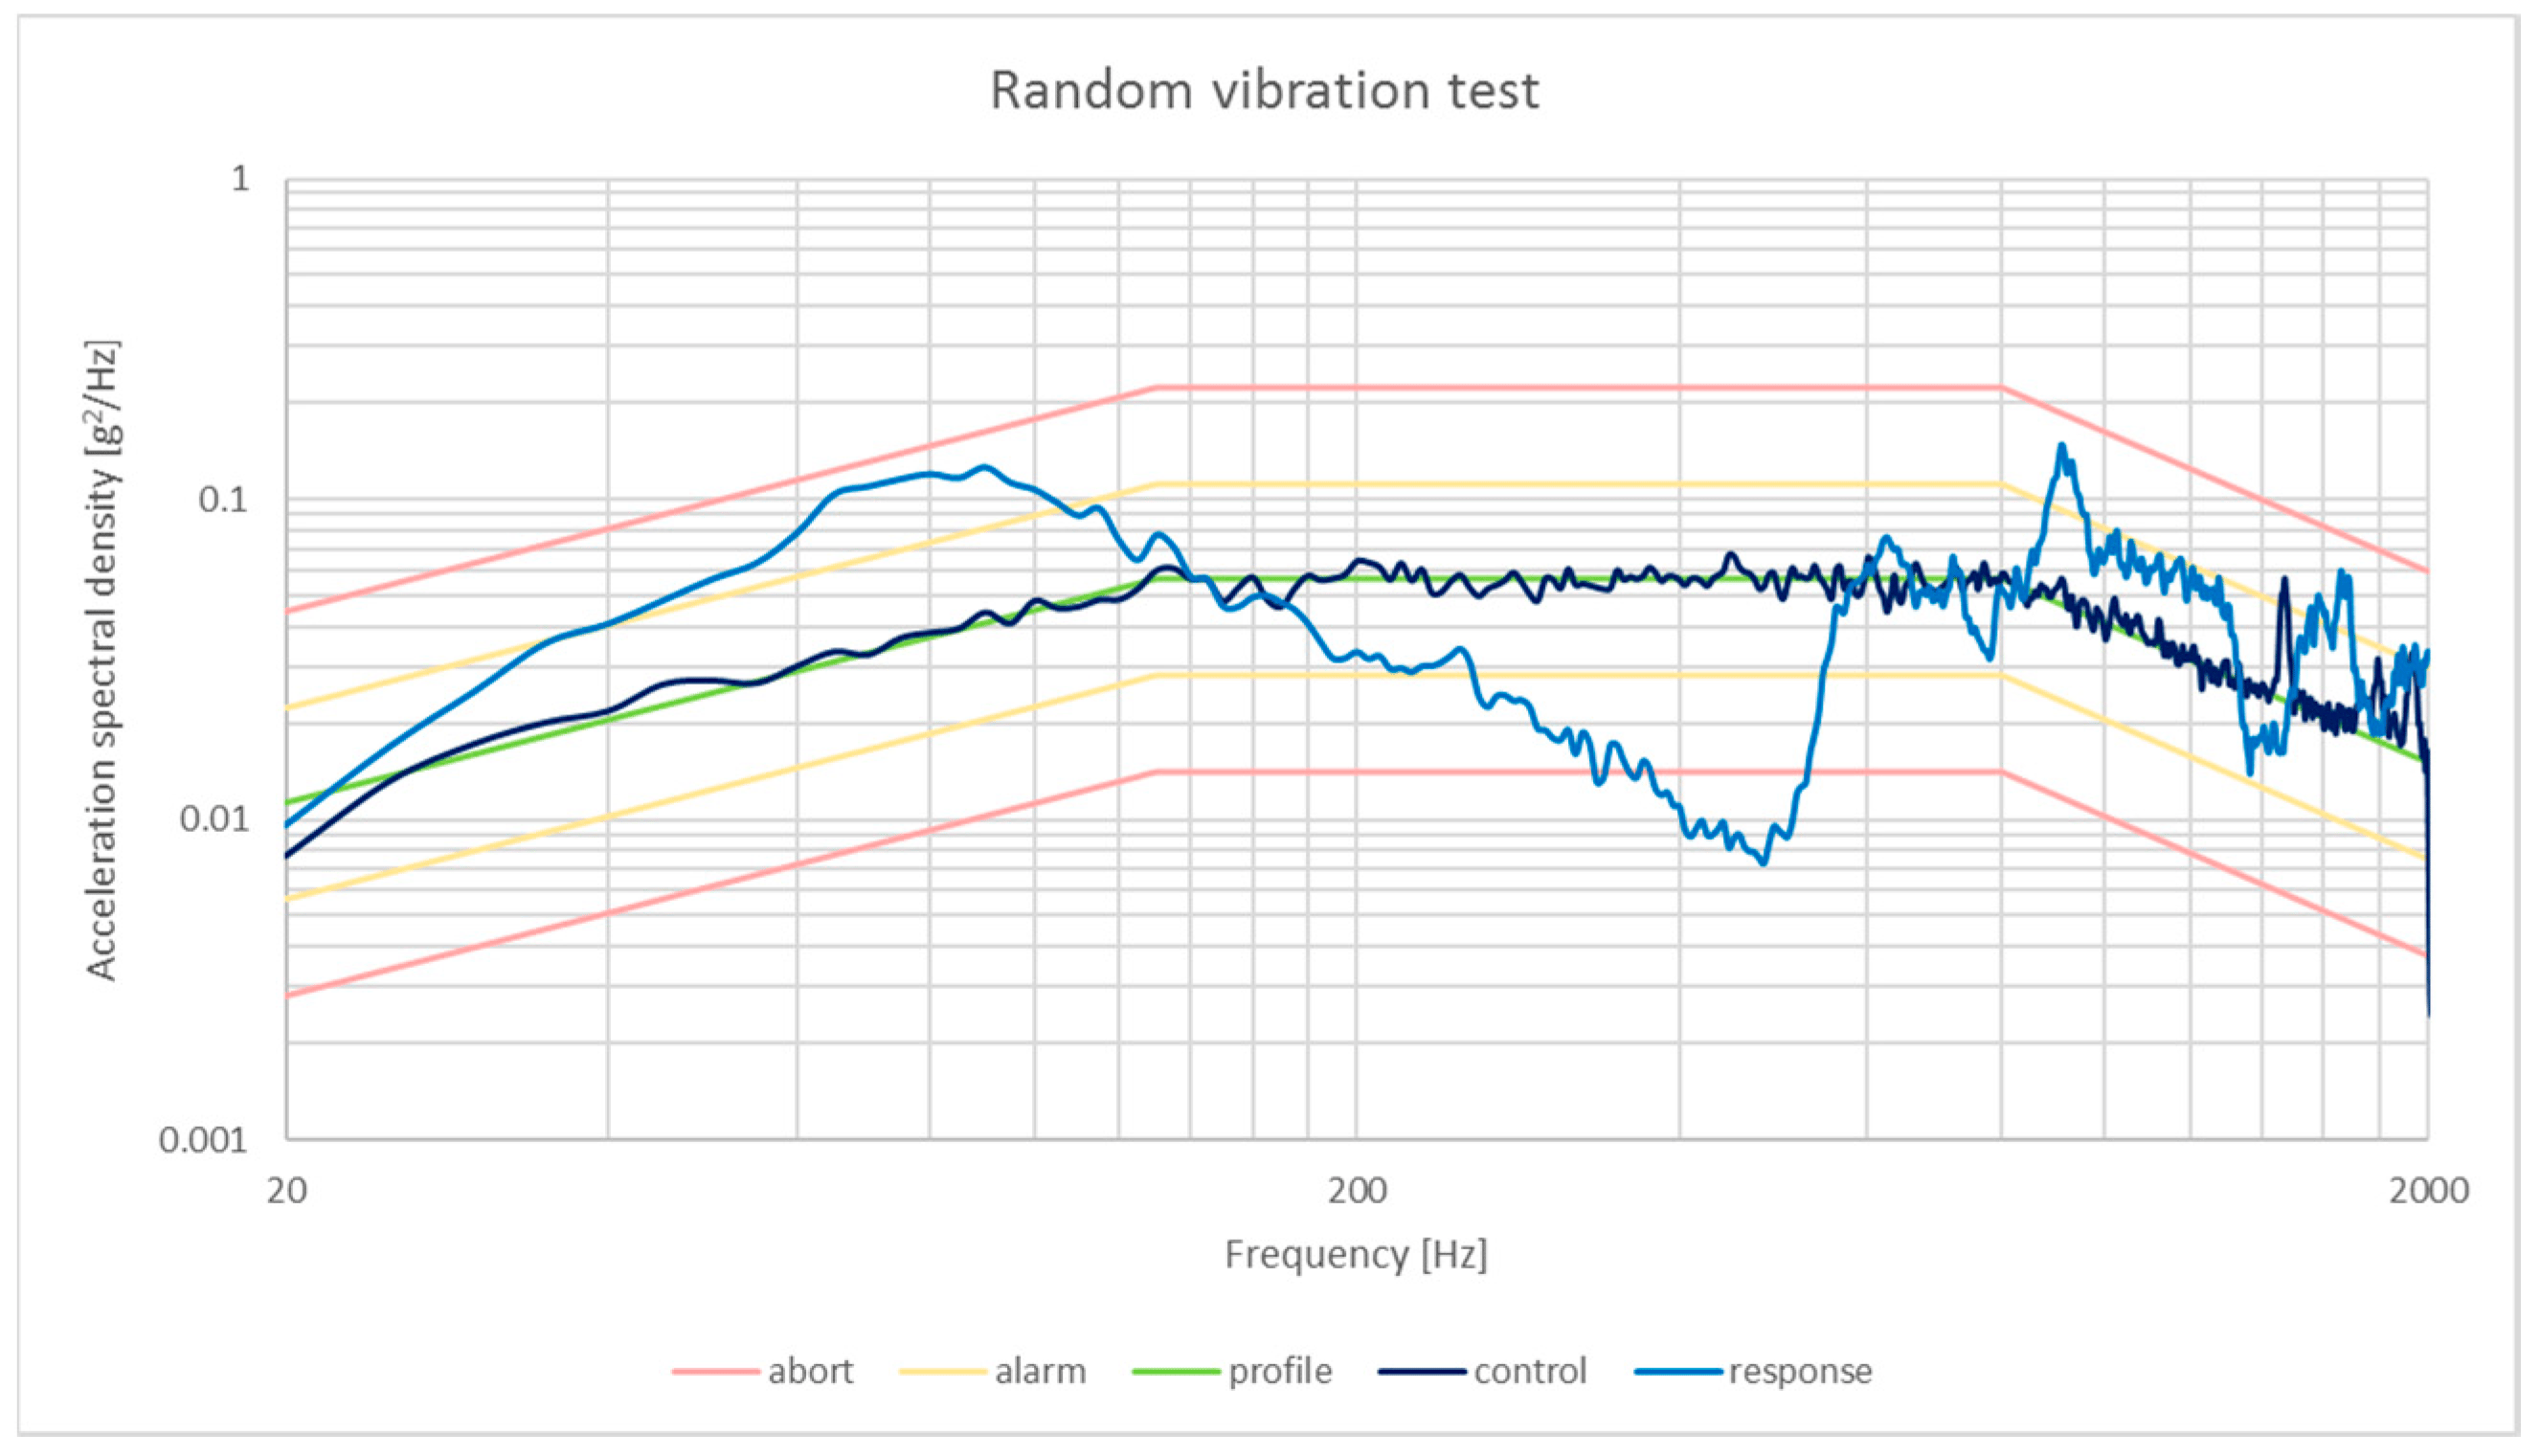
\includegraphics[width=0.75\textwidth]{images/random-study.png}
  \caption{Random vibration test \cite{nieto2019cubesat}}
  \label{fig:random}
\end{figure}

The limitations of random vibration tests is that the shaker and table will have different modes than the launch vehicle and payload mount, resulting in the test response not perfectly matching the flight response \cite{gordon2015benefits,aglietti2019spacecraft}. Gordon and Kern argue that this difference is not a factor in practice since shaker tests are "not intended to be a strength test"  \cite[p.~7]{gordon2015benefits} and that components "should have been strength qualified prior to integration" \cite[p.~7]{gordon2015benefits}. Component level is argued as a best practice in the CubeSat community \cite{rawsonbest}, however some argue that component level testing is not suited to the short timeline of university CubeSat projects and that more effort should be put into integration testing \cite{decker2016systems}. If a testing program focuses on integration testing, then this mismatch between shaker table and flight response could result in the CubeSat not being properly qualified.

Finally, although 6 degrees of freedom (DOF) vibration tables exist which can replicate the vibrations experienced in all dimensions during launch, most satellites are still tested with single-axis or random input shakers which only provide one dimension \cite{gordon2015benefits,aglietti2019spacecraft,nath2022study}. While Gordon and Kern \cite{gordon2015benefits} state that these limitations are adequately managed by testing in all three orthogonal axes separately, Aglietti and Nath \cite{nath2022study} created a model of three, two and single axis vibration tests and found that to match the 3 DOF response with a single DOF table, the satellite needed to be subjected to 2.5 times the $g_\text{rms}$ forces than in 3 DOF testing, leading to the satellite being over designed \cite{nath2022study}.




\subsubsection{Quasi-static acceleration test (QAT)}
A quasi-static test replicates the liftoff stage of flight, where there is a combination of random vibration from engines and quasi-static axial acceleration from the engine and other external forces on the launch vehicle \cite{nieto2019cubesat,brown_elements_2002}, which are approximated as constant forces at selected frequencies as shown in figure \ref{fig:qatforces}. The QAT is usually compared to results from coupled loads analysis, where all forces are assumed to be applied to the satellite through the launch vehicle as shown in figure \ref{fig:cla} \cite{dickens2001coupled}.

\begin{figure}[H]
  \centering
  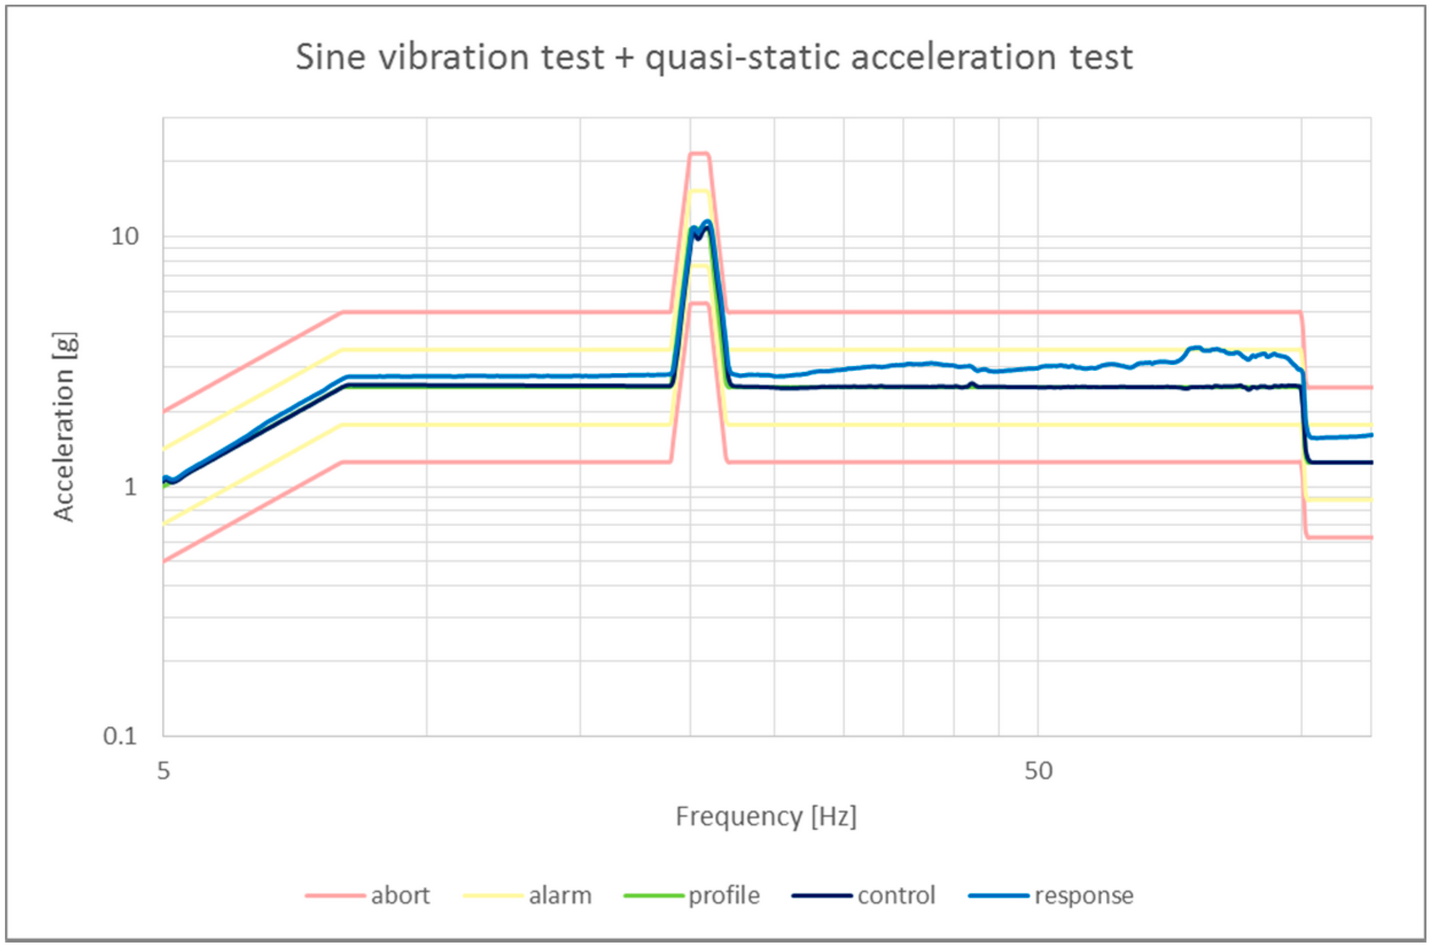
\includegraphics[width=0.75\textwidth]{images/qat.png}
  \caption{Quasi-static acceleration test. The input profile high acceleration from $\SI{20}{\hertz}$ to $\SI{21}{\hertz}$, resulting in the response having a force of 10.8 \textit{g} acceleration around this frequency \cite{nieto2019cubesat}}
  \label{fig:qatforces}
\end{figure}

\begin{figure}[H]
  \centering
  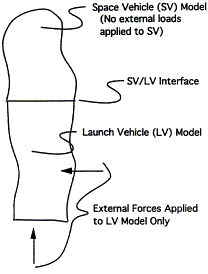
\includegraphics[width=0.3\textwidth]{images/cla.png}
  \caption{Coupled loads model \cite{dickens2001coupled}}
  \label{fig:cla}
\end{figure}

The first limitation of a quasi-static acceleration test is that the shaker table cannot apply the peak response evenly on the CubeSat that is predicted by coupled loads analysis (CLA) \cite{gordon2015benefits}. Again, Gordon and Kern state that these limitations are addressed by component-level strength qualification. They also state that applying the peak response evenly is not necessary, since if an item does not fail, the correctly applying the response evenly does not greatly increase its likelihood of failing \cite{gordon2015benefits}.
The second limitation is there is a difference in modes, since a quasi-static acceleration test also contains random vibrations \cite{gordon2015benefits}.



\subsection{Vibroacoustic testing}

As stated, low frequency vibrations from $\SI{0}{\hertz}$ to $\SI{100}{\hertz}$ tend to couple well through the payload mount, however high frequency vibrations above $\SI{100}{\hertz}$ are more efficiently imparted on the satellite acoustically \cite{gordon2015benefits}. These acoustic loads have an effect on payload electronics \cite{casalino2012rocket}, and primarily originate from the highly turbulent engine exhaust \cite{casalino2012rocket}.

Vibroacoustic testing is not necessary for CubeSats due to their small surface area \cite{nasa-gevs}, since the magnitude of the acoustic response is proportional to the satellite's surface area to mass ratio \cite{brown_elements_2002}, therefore the effect of the acoustic loads is negligible. Instead, vibroacoustic testing is more relevant for large and light payloads such as solar panel arrays \cite{brown_elements_2002}, therefore it will not be part of this research.

\subsection{Shock}

Shock is experienced by satellites when pyrotechnics are detonated or deflagrated during events such as staging and ignition, the response appears as a range of decaying sinusoids in the $\SI{100}{\hertz}$ to $\SI{10}{\kilo\hertz}$ frequency range \cite{brown_elements_2002}, which decay in $\SI{5}{\milli\second}$ to $\SI{15}{\milli\second}$ \cite{brown_elements_2002}. The spectrum extends up to $\SI{40}{\kilo\hertz}$, however for analysis frequencies above $\SI{10}{\kilo\hertz}$ are assumed to be non-damaging \cite{bement1995manual,nasa-pyroshock}. Pyroshock may cause peak accelerations of up to 10000 \textit{g} \cite{nasa-pyroshock}. High explosives are primarily used for explosive elements on rockets in combination with some low explosives for initiators \cite{bement1995manual}.

Shock is tested using a shock-generating device which is applied to the satellite along all three axes \cite{nasa-gevs,nasa-pyroshock}, the shock generating device for a CubeSat can be an electrodynamic shaker table \cite{nieto2019cubesat} with a half-sine, pulse profile \cite{nieto2019cubesat}. The shock test has similar limitations as the random vibration test, since it also uses a vibration table to affect the satellite.

Shock tests are compared using the shock response spectrum (SRS), which plots the maximum acceleration per frequency bin. The SRS contains an octave slope which rises to the first resonant frequency called the "knee frequency". The octave slope can be approximately 9 dB/octave to 12 dB/octave depending on distance to the source.

\begin{figure}[H]
  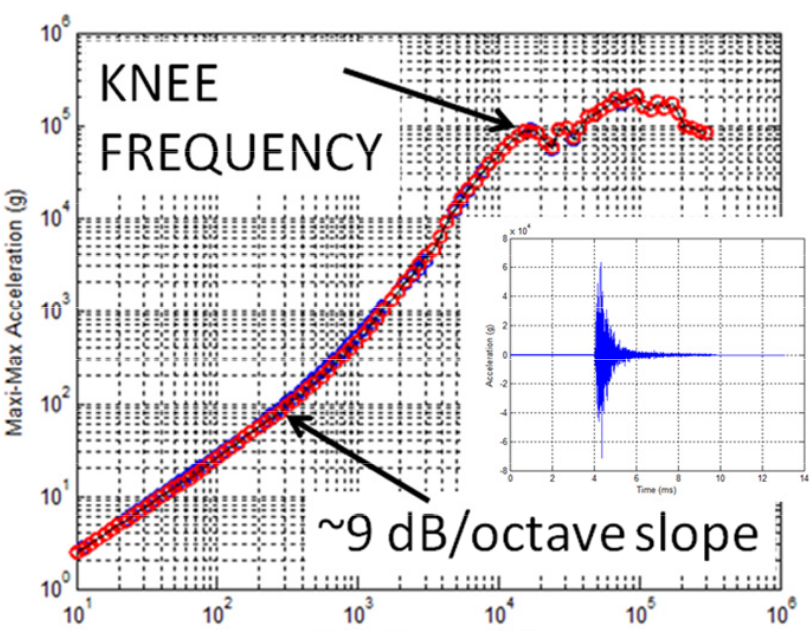
\includegraphics[width=0.5\textwidth]{images/pyroshock2.png}
  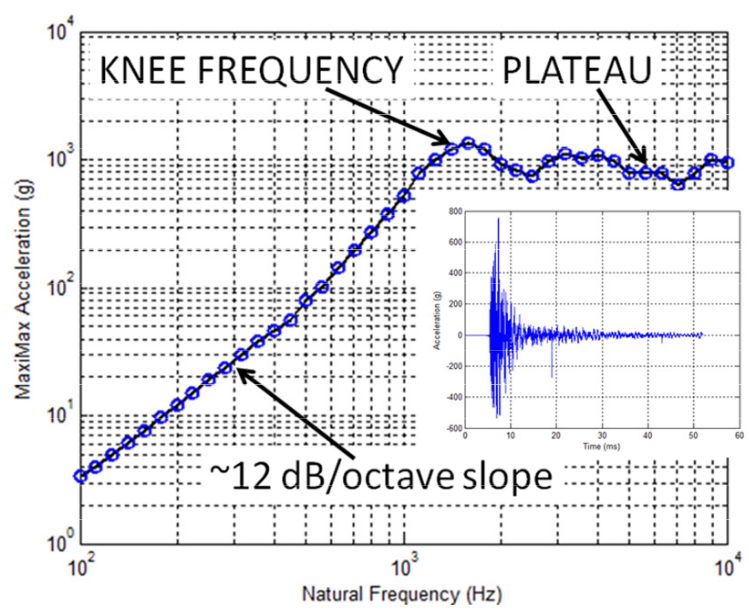
\includegraphics[width=0.5\textwidth]{images/pyroshock1.png}
  \caption{Shock response spectrum of and time-domain shock response. Left: near-field (close to shock source). Right: far-field (distant from shock source) \cite{nasa-pyroshock}}
  \label{fig:pyroshock}
\end{figure}


\subsection{Rocket testing of CubeSats}
\subsubsection{Sounding rockets}
Sounding rockets are a class of suborbital rocket used between $\SI{40}{\kilo\meter}$ and $\SI{200}{\kilo\meter}$, above where weather balloons operate \cite{seibert2006history}. While sounding rockets have been used to launch many CubeSats as the primary launch vehicle for suborbital CubeSat missions, such as in the REXUS-25 mission \cite{pont2019rexus}, there has been only one published instance of sounding rockets being used as an additional qualification platform for a CubeSat \cite{slongo2019pre}. The FloripaSat-I CubeSat was tested on a VSB-30 sounding rocket \cite{slongo2019pre} to qualify the CubeSat under launch conditions. This qualification method was intended not to replace, but to complement standard vibration and shock qualification methods \cite{slongo2019pre}. The test measured these launch conditions through the MPU6050 6 DOF inertial measurement unit (IMU) \cite{slongo2019pre}.

\begin{figure}[H]
  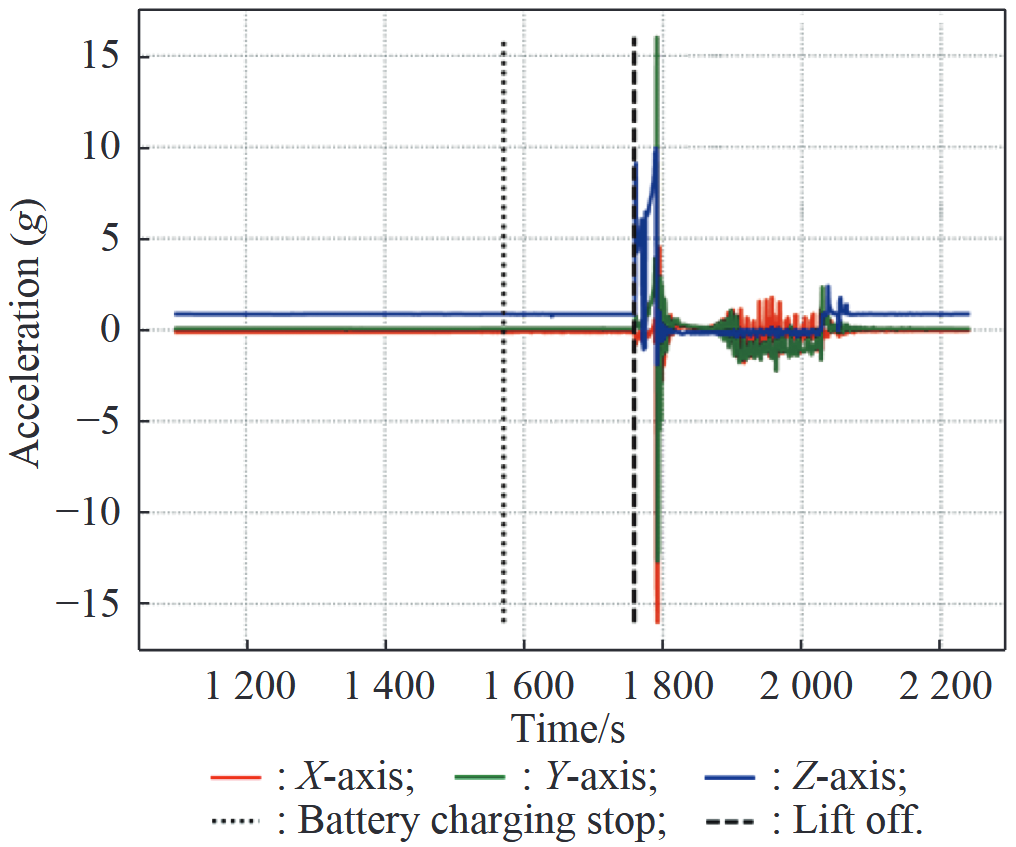
\includegraphics[width=0.5\textwidth]{images/floripa-accel.png}
  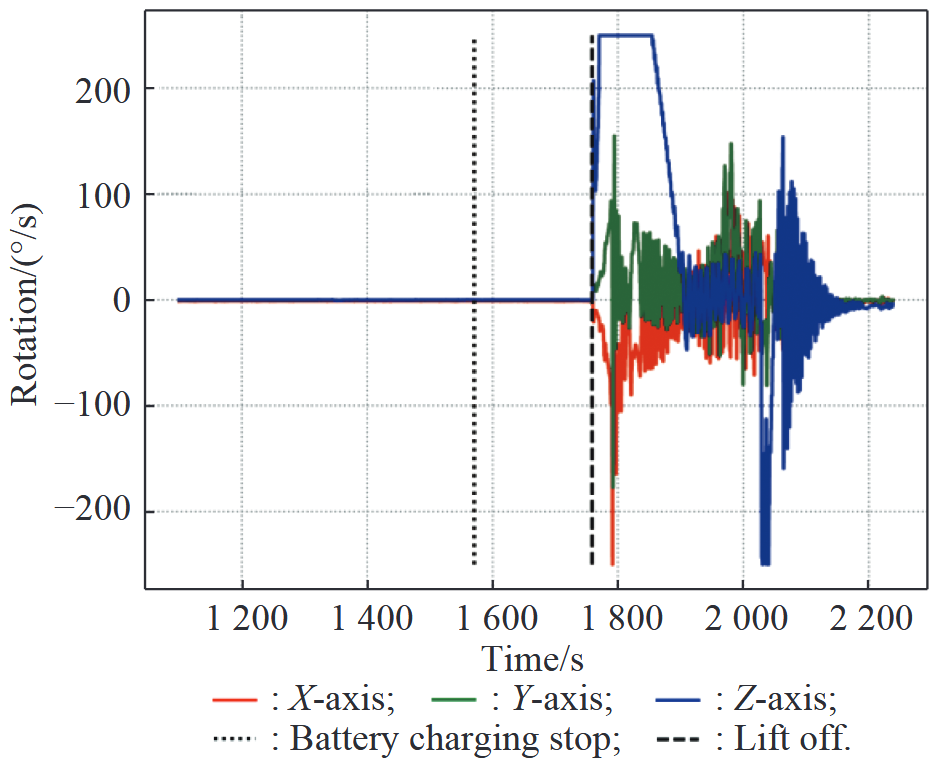
\includegraphics[width=0.5\textwidth]{images/floripa-rot.png}
  \caption{Acceleration in time domain (Left), Angular velocity in time domain (Right) during the launch of FloripaSat-I \cite{9316404}}
  \label{fig:accel-rot}
\end{figure}

While this study does show the time-domain accelerometer and gyroscope measurements from the sounding rocket launch in figure \ref{fig:accel-rot}, it does not compare the data to other qualification tests in the FloripaSat-I campaign, such as traditional vibration and shock testing. Additionally, the launch data was not presented in the frequency domain through the boost and coast phases of the flight, meaning they could not be compared to the acceleration spectra which was shown for the shaker table testing in figure \ref{fig:shaker}.

\begin{figure}[H]
  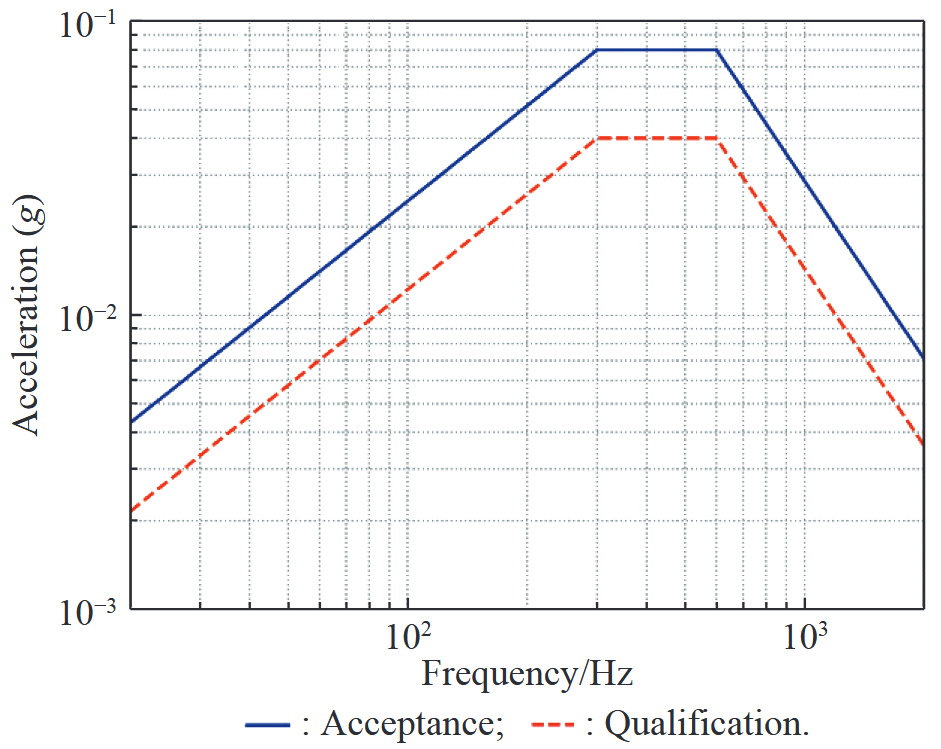
\includegraphics[width=0.5\textwidth]{images/floripa-random-spectrum.png}
  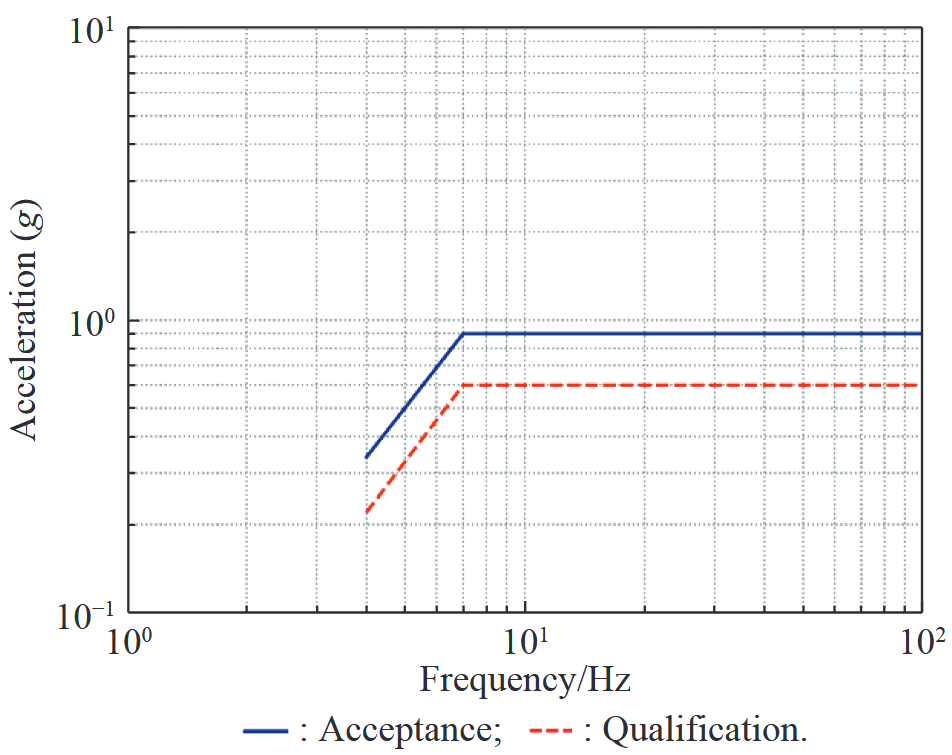
\includegraphics[width=0.5\textwidth]{images/floripa-sinusoid.png}
  \label{fig:shaker}
  \caption{Random vibration (Left) and sine sweep (Right) tests on a shaker table during the qualification of FloripaSat-I \cite{9316404}}
\end{figure}

Another shortcoming of the study is that a shock test using a half-sine pulse was not performed. The use of a sounding rocket is a potential method of qualifying the CubeSat's ability to tolerate shocks since there will be shock events when pyrotechnics are lit to stage the rocket, although the forces will have intensity than on a larger launch vehicle.

\subsubsection{High-power rockets (HPR)}
While sounding rockets have a significantly lower cost compared to an orbital-class launch vehicle, they cost \$1 million USD per launch to launch $\SI{200}{\kilo\gram}$ on average \cite{jurist2009COTS}, resulting in a specific cost of \$5000 USD/kg, which is still a large amount for university CubeSat programs. High-power rockets (HPR) are a lower-performance but cheaper alternative to sounding rockets, which can leverage the design expertise of university rocketry teams while having similar qualification potential as sounding rockets. A single stage level 3 certification rocket can reach altitudes above $\SI{10000}{\feet}$ \cite{canepa2005modern} for a cost of only \$1200 USD \cite{canepa2005modern}. Despite the potential cost benefits, there have not been any published instances of a HPR being used to qualify a CubeSat.

The typical phases of a HPR launch are

\begin{itemize} % TODO: FIND SOURCES FOR THIS SECTION
  \item Boost phase: The HPR is being powered by a solid rocket motor. In most HPR launches, this phase only lasts several seconds at maximum.
  \item Coast phase: After the rocket motor burns out and produces no thrust the rocket coasts up on a ballistic trajectory to the maximum altitude (the apogee).
  \item Apogee: This is the maximum altitude the rocket will reach. At this point the drogue parachute is deployed, which limits the rocket's descent velocity to a reasonable rate %TODO: WHat?
  \item Main parachute deployment: At a fixed altitude above ground level the main parachute is deployed. This parachute has a higher surface area than the drogue chute and slows the rocket down to a safe landing velocity. A main parachute should not be deployed at apogee since this would result in the rocket drifting further which complicates recovery efforts.
  \item Landing: The rocket lands on the ground and is recovered by the rocketry team for safing (disarming of live energetics) and transportation. While the landing occurs minutes after launch, finding the rocket is a harder task and may occur hours after landing.
\end{itemize}

\begin{figure}[H]
  \centering
  \includesvg[width=0.75\textwidth]{images/rocket_graphic.svg}
  \caption{Typical launch of a single stage high-power rocket}
  \label{fig:rocket_flight}
\end{figure}

One potential issue with HPRs as a qualification platform for shock is that low explosive black powder is used \cite{canepa2005modern} which has different explosive characteristics, such as a subsonic flame front, compared to the high-explosives used in launch vehicles \cite{bement1995manual} and will therefore produce different shock responses. One study \cite{wang2023numerical} performed finite element analysis of igniters filled with low explosives including aluminium potassium perchlorate and boron potassium nitrate and determined the SRS, shown in figure \ref{fig:lowsrs}. Compared to the SRS of high-explosives in figure \ref{fig:pyroshock}, where at a frequency of 1 kHz the acceleration is over $10^2$ \textit{g} \cite{nasa-pyroshock}, in these low explosive simulations the acceleration at 1 kHz is only $10^1$ \textit{g} \cite{wang2023numerical}. Therefore, it is hypothesised that HPRs will not be useful for shock qualification since the response of low explosives is different from the high explosives used on launch vehicles.


\begin{figure}[H]
  \centering
  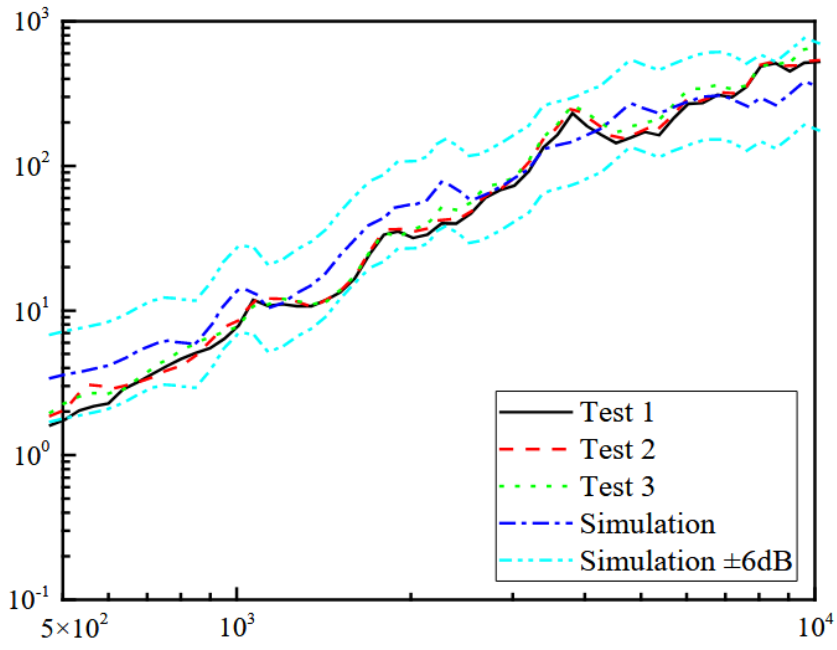
\includegraphics[width=0.75\textwidth]{images/deflagration.png}
  \caption{Shock response spectrum from computer modelling of an igniter based on the low explosive aluminium potassium perchlorate \cite{wang2023numerical}}
  \label{fig:lowsrs}
\end{figure}

% Project Process – Design Process
% The design process should be described in sufficient detail to permit readers
% to understand the approach used to arrive at the final design. This should
% include;A description of the constraints imposed on the design; Descriptions
% of any design tools employed; A discussion of the relevant code sections or
% requirements; A framework for evaluating the success of the resulting design.

\section{Project overview}



% \section{Design constraints}
\section{Design group}

The CubeSat design group was made of Peter Tanner, Jamir Khan and Timothy Ludovico. As shown in figure \ref{fig:cubesat-responsibilities}, each person is working on a unique part of the CubeSat and requires specific information to be communicated.

\begin{figure}[H]
  \centering
  \includesvg[width=0.75\textwidth]{images/project_hierarchy.svg}
  \caption{Responsibilities of members on the CubeSat design project and the information required to be communicated between each member.}
  \label{fig:cubesat-responsibilities}
\end{figure}

% \begin{table}[H]
% \centering
% \begin{tabular}{|c|p|p|}
%   Person &  Responsibilities & Information required to complete section \\
%   \hline
%   Peter Tanner      & Design and build of POEM emulation electronics and data acquisition system  & Jamir: \\
%   Jamir Khan        & Design and build of HPR and CubeSat body, integration of CubeSat in HPR     & \\
%   Timothy Ludovico  & Design and build of camera array, integration of optics                     & \\
% \end{tabular}
% \caption{Design group responsibilities}
% \label{tabl:design-group}
% \end{table}



\section{Design tools}

\subsection{Altium Designer 24}

Altium Designer is an electronics design automation (EDA) tool which is widely used in industry and has been used for design of CubeSat and space hardware \cite{10061409}. %TODO: wording (personal language?)
The author chose to use Altium Designer over other EDA tools since they were familiar with this tool having used it in previous projects, which minimises development time.

The design flow in Altium designer is as follows:
\subsubsection{Schematic editor}
A circuit is first implemented using schematic symbol representations of components in the schematic editor. In the schematic view the connections between the components are abstracted using net labels and wires. The schematic view does not necessarily represent the physical layout of the PCB but is intended to convey the connections between components in a format that can easily be read.



\begin{figure}[H]
  \centering
  \includesvg[width=0.75\textwidth]{images/altium_schematic_hierarchy_example.svg}
  \caption{Example of the hierarchical schematic sheet format for the main DAQ PCB.}
  \label{fig:altium-schematic-hierarchical}
\end{figure}

A root schematic contains references to other schematics which are abstracted as sheet symbols with ports. Each sheet symbol represents a particular subsystem of the DAQ. The hierarchical sheet symbol representation has several benefits, including that it facilitates reuse of designs and allows larger systems to be decomposed into multiple schematics which are easier to modify and read. This is shown in figure \ref{fig:altium-schematic-hierarchical}.


\subsubsection{PCB editor}
Each schematic symbol is a component which links the symbol to a footprint. The footprint is the physical representation of the component and contains information such as
\begin{itemize}
  \item The land pattern, which is the layout of pads or holes required for mounting the component on the PCB,
  \item The component's 3d model
\end{itemize}

The PCB editor contains automated design rule check (DRC) tools which is used in the design process to reduce the likelihood of a faulty PCB. The DRC uses rules set in the project and if a rule is violated, it is reported. This feature is used for example to ensure that microwave-frequency tracks have the correct geometry for impedance matching.

\subsubsection{Output jobs}
Once a PCB is ready to be manufactured, an automated "outjob" ensures that the required design files are automatically generated with the right settings for manufacturing. The files generated include:
\begin{itemize}
  \item Bill of materials
  \item Gerber files
  \item Drill location files
  \item Pick-and-place component locations
\end{itemize}


The outjob feature prevents errors such as misconfiguration of output files.


\subsection{circuit.js}

Circuit.js is a simple browser-based analog circuit simulator \cite{falstad22falstad}. Circuits in this simulator can be edited and interacted with in real-time, whereas in traditional SPICE simulators the circuit cannot be edited once the simulation starts. Circuit.js uses a numerical method which is prone to error however, therefore this simulator was used for rapid, real-time prototyping of designs. After these designs were finalised they were simulated in traditional SPICE-based simulators.

\subsection{LTspice}

The simulation of components is done using LTspice, a freeware circuit simulator which uses the SPICE method

LTspice was used to the DC-DC boost converter for this project, which was required to power the internal DAQ systems and the payload. A simulation was performed to characterise the ripple voltage and to validate its performance over a range of input voltages. LTspice has been used for simulation of boost converters in the past and is free which makes it a suitable circuit simulator for this project \cite{giesselmann2019modeling}.

Ultimately LTspice was chosen over other freeware SPICE simulators such as PSpice since LTspice contains an "alternate" solver which has less error at the trade-off of simulation time \cite{ltspice2022}. The reduced error results in the solver converging on a solution, whereas in PSpice or in LTspice normal solver mode it was not able to converge on a solution and the simulation could not be completed.

\subsection{SolidWorks 2023}
SolidWorks is a mechanical CAD software which is used for creating 3d models of the electronics hardware by using the Altium Designer plugin. These 3d models are required for Jamir to complete the mechanical design of the CubeSat and to verify good mounting of the electronic hardware.

\section{Design process}

\subsection{Identification of constraints and requirements}
\label{sec:constraints-and-requirements}

The beginning of the design process involves identification of constraints and requirements.

The ultimate goal of this testing campaign is to receive at least one image from the camera payload from a drone or HPR flight, and launch on the POEM and receive at least one image from orbit. The POEM will remain in low Earth orbit (LEO) for 6 months \cite{jagdale2023sanket}.

\subsubsection{Electrical power system (EPC) requirements and constraints}
\paragraph{Battery life} POEM outputs a consistent amount of power to each CubeSat while on orbit due to its solar panels and battery system, however in the tests it will not be possible to deploy a solar panel therefore the DAQ system must have adequate battery life to power the camera payload throughout the length of the test.
\paragraph{Voltage and current} A requirement of the EPC on the DAQ is to emulate the voltage and current provided by the POEM to one CubeSat to facilitate testing of the camera payload's power electronics. POEM contains a \SI{28}{\volt} and \SI{42}{\volt} bus, however IIST has informed the design team that a \SI{5}{\volt} connection with a maximum current of \SI{1.5}{\ampere} is provided to CubeSats. The EPC will have to emulate at least one of these power busses.

\subsubsection{Environmental requirements}
It is possible a future version of this payload will fly with the camera payload on POEM to make a direct comparison between the vibration environment on POEM to the conditions on both a HPR and the shaker table tests. Therefore, the DAQ must go through the same qualification campaign as the camera payload.

\paragraph{Shock, random vibration, sine-sweep test pass} The DAQ must remain functional during the vibration environment of the rocket. This means it must pass the IIST recommended qualification procedure, which involves shock, random vibration and sine-sweep tests. These tests are described in more detail in section \fullref{sec:shaker-table-test}.

\paragraph{Cold and hot temperature test pass} The DAQ must be able to survive at temperatures of \SIrange{-20}{80}{\degreeCelsius} as described in section \fullref{sec:htemp-test-framework} and section \fullref{sec:ltemp-test-framework}. This will influence the components that can be used.
\subsubsection{Physical requirements}

\paragraph{Physical dimensions} The DAQ must have physical dimensions that allow it to fit within the inside space of a 1U CubeSat.

\subsubsection{HPR test requirements}

\paragraph{GNSS tracking} In the original plan, the HPR will launch to a high altitude and may drift away from the launch site. Tracking of the CubeSat will be required to ensure recovery.

\paragraph{Radio link range} One of the key requirements stated was receiving one image from a drone or HPR flight. This requires a stable radio link with a protocol that allows the received image to be recognisable even if the link degrades.


\subsection{Parts selection and constraints}

The first part of the design process is to obtain a list of constraints and requirements for the DAQ system, and from these constraints choose appropriate components to achieve the requirements.

The small payload size and recovery sequence of the HPR presents unique constraints for this data acquisition system, which prevented the use of COTS off the shelf (COTS) DAQs and sensors.

\subsubsection{Experimental requirements}

This project in addition to design of a DAQ involves design of an experiment to evaluate both HPR launches and shaker tables as comparable qualification platforms to the IIST recommended qualification level.

\paragraph{Sampling rate} The accelerometers used must be able to sample at twice the frequency bandwidth of the tests. This is to avoid sampling according to the Nyquist criterion.

\paragraph{Maximum measurable acceleration} Pyroshock events and motor launch are high-\textit{g} events that require accelerometers with measurement scales above these events, otherwise they will saturate at the maximum scale.

\subsubsection{Other requirements}

\paragraph{2024 Australian Universities Rocket Competition (AURC) regulations} This payload was intended to fly on the UWA Aerospace rocket \textit{Svengeance} in the AURC 2024 competition, as part of a collaboration with UWA Aerospace. AURC has additional rules for electronics systems, relevant rules include (but not limited to) \cite{ayaa2023specifications}:
\begin{itemize}
  \item Lithium-polymer batteries are not allowed (unless using COTS equipment)
  \item Connectors must have a positive locking mechanism
  \item Electronics must be mounted using rigid fixing methods
\end{itemize}

\paragraph{Budget} The cost of the DAQ system must not exceed \$AU 1500.

% \begin{table}[H]
% \centering
% \begin{tabular}{|c|p{0.3\linewidth}|p{0.3\linewidth}|}
%   Constraint &  Definition  & Reason required\\
%   \hline
%   Battery life  & The amount of time (hours) that the DAQ will be active for  & DAQ has to be active through the pre-launch time, launch and for long enough after launch to facilitate tracking of the rocket for recovery. \\
%   Sampling rate & The number of samples the DAQ takes per second of the accelerometer data & Analysis of random vibration and shock data involves constructing a power spectral density plot of the accelerometer data, which requires the DAQ to sample at a frequency greater than twice the plot frequency range. \\
%   Accelerometer range & Accelerometers have a maximum acceleration that can be measured before it saturates at the maximum magnitude. An accelerometer with a high acceleration range is required for high-\textit{g} events such as pyroshock. \\
%   Storage size & The number of bytes available on the DAQ for accelerometer data to be stored. \\
%   Radio link range  & Line-of-sight (LOS) distance in meters that the DAQ must be able to relay data to the ground station  & Drone tests require live image data for positioning purposes. \\
%   Power supply & The DAQ must be able to provide the same voltage and current as POEM (). & The camera payload is built assuming power is provided by the POEM\\
%   Form factor  & Dimensions of the data acquisition system & It must fit inside the CubeSat \\
%   Temperature ruggedness & The DAQ must survive temperatures ranging from \SIrange{-20}{80}{\degreeCelsius} & 
%   % Test Price & The amount of money required to construct the DAQ & \$1500 has been allocated to this part of the project.\\
%   % Temperature tolerance & The maximum and minimum temperature the DAQ can operate at & The DAQ will be tested in the same conditions as the camera payload during its temperature tests.\\
% \end{tabular}
% \caption{Design constraints for the DAQ System}
% \label{tabl:design-constraints}
% \end{table}

\subsection{Selection of components}

The constraints in section \fullref{sec:constraints-and-requirements} will determine the parts that are appropriate for the design.

\paragraph{Battery selection}

Commercial off the shelf (COTS) 18650 lithium-ion batteries were chosen due to the following features:

\begin{itemize}
  \item H
  \item High specific energy \cite{krause2021performance}.
\end{itemize}

COTS 18650 lithium-ion batteries were chosen as the energy source for the DAQ. Advantages of this battery format include:

\begin{itemize}
  \item The 18650 format encases the battery in a rigid metal cylinder which is well-suited for the space environment \cite{knap2020review}. Battery formats which use a flexible pouch, like most lithium-polymer cells, are more prone to outgassing in the vacuum of space \cite{knap2020review}. 
  \item Compared to other rechargeable battery solutions such as \ce{Ni}-\ce{Cd} and \ce{Ni}-\ce{H2}, \ce{Li}-ion batteries have improved temperature range, energy density and specific energy and cycle life \cite{pathak2023review}.
  \item COTS \liion batteries are a mature battery format due to widespread use in consumer products \cite{pathak2023review}.
  \item Extensive flight heritage as they have been proven in other CubeSat missions \cite{knap2020review}, and are being used on flagship NASA missions, such as Europa Clipper \cite{krause2021performance}.
  \item Low cost as they are COTS grade and are already produced at scale. % TODO: Citation
\end{itemize}

% TODO: MOVE TO FINAL DESIGN SECTION
Manufacturers produce a variety of types of \liion batteries with different chemistries, which affect parameters including internal resistance, discharge and charging temperature range and capacity.

The Samsung INR18650-25R \liion battery was chosen for the DAQ platform due to
\begin{itemize}
  \item Previous flight heritage on CubeSats \cite{marcelino2021orbit}.
  \item Operation over a large temperature range of \SIrange{-20}{75}{\degreeCelsius} and has been proven to be stable at \SI{130}{\degreeCelsius} \cite{samsung2014}.
  \item Good capacity of \SI{2500}{\milli\ampere\hour} and high maximum discharge rate of \SI{20}{\ampere}.
\end{itemize}

Three batteries were placed in parallel to form a 1S3P battery pack, this configuration was chosen as it simplifies the charging circuitry by removing the need for cell balancing circuitry that is required for series battery packs, which reduces cost and simplifies the design. Three cells were selected since this %TODO: justify 1S3P capcity.
% TODO: MOVE TO FINAL DESIGN SECTION

\paragraph{Power electronics} Power electronics are used to stabilise the battery voltage, since a \liion battery may have a voltage ranging from \SIrange{4.2}{2.5}{\volt} over one discharge cycle.

\begin{table}[H]
\centering
\begin{tabular}{|c|c|c|c|c|}
  \hline
  \textbf{Item}  & \textbf{Voltage (\si{\volt})} & \textbf{Unit current (\si{\milli\ampere})} & \textbf{Quantity} & \textbf{Current (\si{\milli\ampere})} \\
  \hline
  Payload-under-test & 5 & 1500 (Max.) & 1 & \\
  Raspberry Pi Zero W & 5 & & 1 & \\
  NEO-M9N & 3.3 & & 1 & \\
  ZED-F9P & 3.3 & & 1 & \\
  LSM6DSOX & 3.3 & & 2 & \\
  ADXL375 & 3.3 & & 2 & \\
  % ADXL375 & 3.3 & & 1 & \\
  E32-900M30S & 3.3 & & 1 & \\
  % TODO: RS-485, SC16I750, 
  \hline
  % \textbf{Total}  & - & \\

\end{tabular}
\caption{Operating voltage and current consumption of devices connected to EPC.}
\label{tabl:epc-power-budget}
\end{table}


\subsection{Implementation of parts into design}

\begin{figure}[H]
  \centering
  \includesvg[width=0.9\textwidth]{images/ecad_workflow.svg}
  \caption{Workflow for integrating a design into a PCB.}
  \label{fig:ecad-workflow}
\end{figure}

% \subsection{Integration testing}

\subsection{Preliminary testing}

These tests were conducted prior to main tests to reduce the risk of failure in main tests and to make a judgement about whether the main test should be conducted or be called off.

\begin{itemize}
  \item Integration testing with camera system % EXample: Found bugs with communications
  \item Ground distance testing % Example: resulted in the development of the block-based transmission protocol
\end{itemize}

\section{Design evaluation framework}

The design evaluation framework will consist of three major types of tests:

\begin{itemize}
  \item Environmental tests.
  \subitem Hot and cold temperature testing.
  \subitem Shaker table.
  \item Vehicle tests.
  \subitem Drone.
  \subitem Rocket.
  \item Experimental evaluation.
  \subitem Evaluation of accelerometers.
\end{itemize}

\subsection{Environmental testing}

%TODO: Make this more obvious earlier on about futrre work
If this research continues, the DAQ will need to fly with the CubeSat on the PSLV to obtain vibration data that can be directly compared to the rocket and shaker table tests. Therefore, the DAQ will have to go through the same environmental testing campaign as the camera payload. The objective of these tests is to evaluate the resilience of the DAQ in the environment of space and during launch.

\subsubsection{High-temperature test}
\label{sec:htemp-test-framework}
IIST recommends a qualification test where the CubeSat placed in a thermal vacuum chamber for $\SI{2.5}{\hour}$ and is heated to $\SI{70}{\degreeCelsius}$. The CubeSat electronics are turned on and tested during the final $\SI{30}{\minute}$ of the test.

Due to time restrictions it was only possible to do a preliminary high-temperature test with a consumer oven on only the electronics section of the payload (the combined camera and DAQ assembly).

\begin{figure}[H]
  \centering
  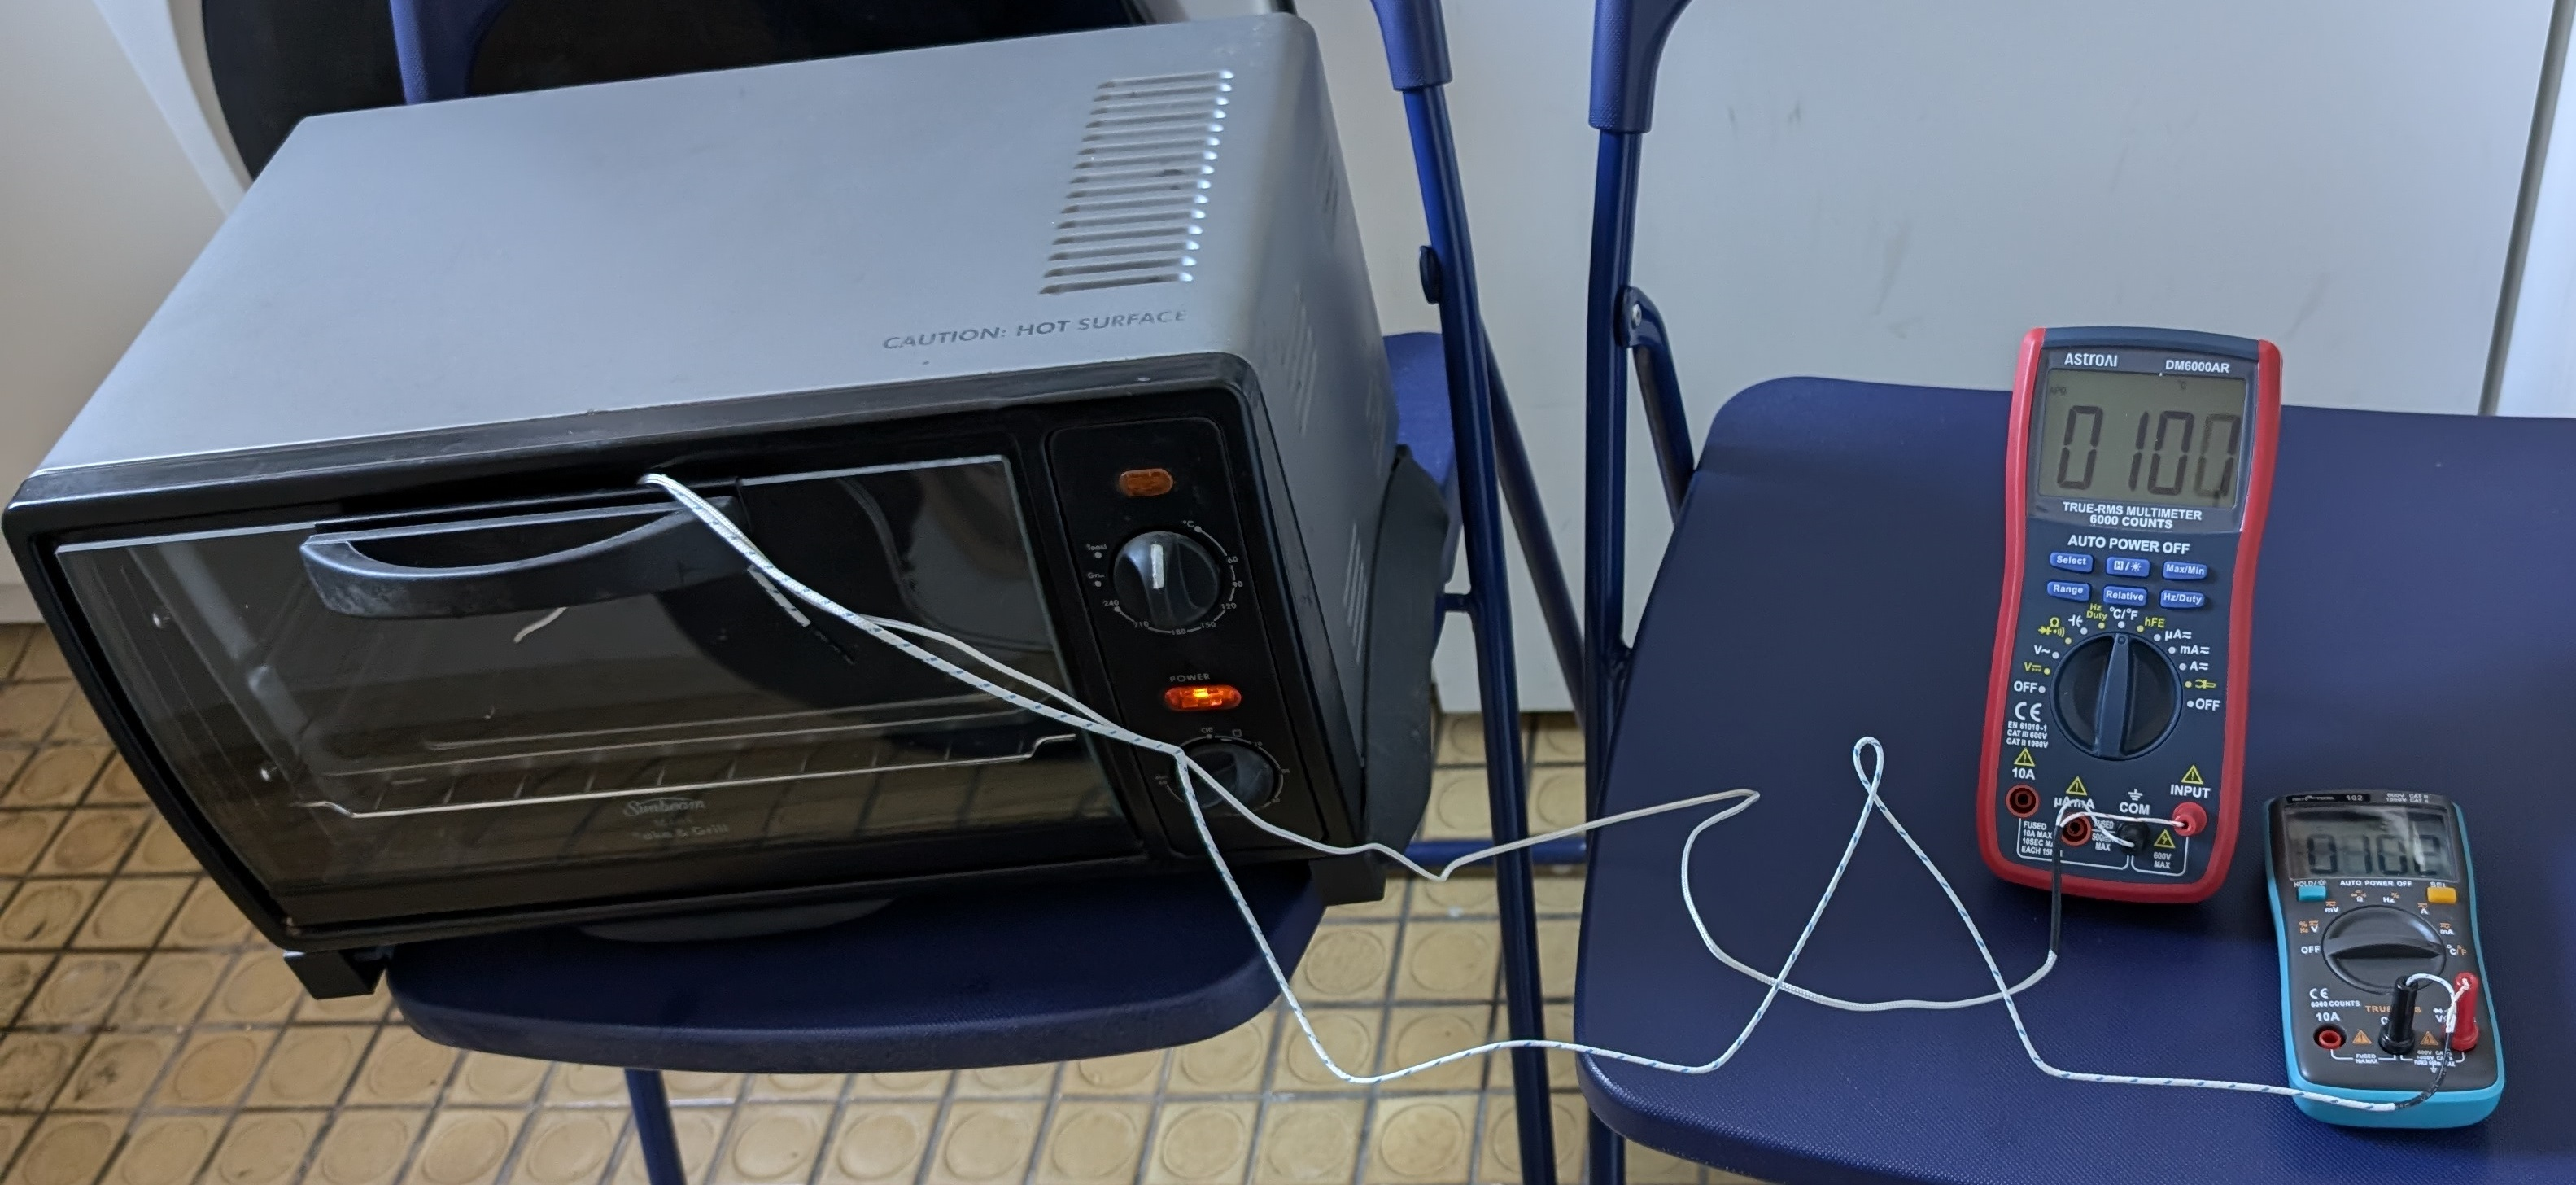
\includegraphics[width=0.75\textwidth]{images/oven_test.jpg}
  \caption{High-temperature testing setup}
  \label{fig:temperature-testing-oven}
\end{figure}

The DAQ was evaluated based on how much time the connection between the DAQ and ground station is lost.

\subsubsection{Low-temperature test}
\label{sec:ltemp-test-framework}
IIST recommends a qualification test where the CubeSat is placed into a thermal vacuum chamber for $\SI{2.5}{\hour}$ and is cooled to $\SI{-20}{\degreeCelsius}$. The CubeSat electronics are turned on and tested during the final $\SI{30}{\minute}$ of the test.

Due to time restrictions it was only possible to do a preliminary low-temperature test with a consumer freezer. To prevent condensation from developing on the electronics during the test, which would not occur in the thermal vacuum chamber, the electronics were placed in an airtight bag prior to the test and pressurised with pure nitrogen gas for $\SI{5}{\minute}$ to displace air containing moisture.

\begin{figure}[H]
  \centering
  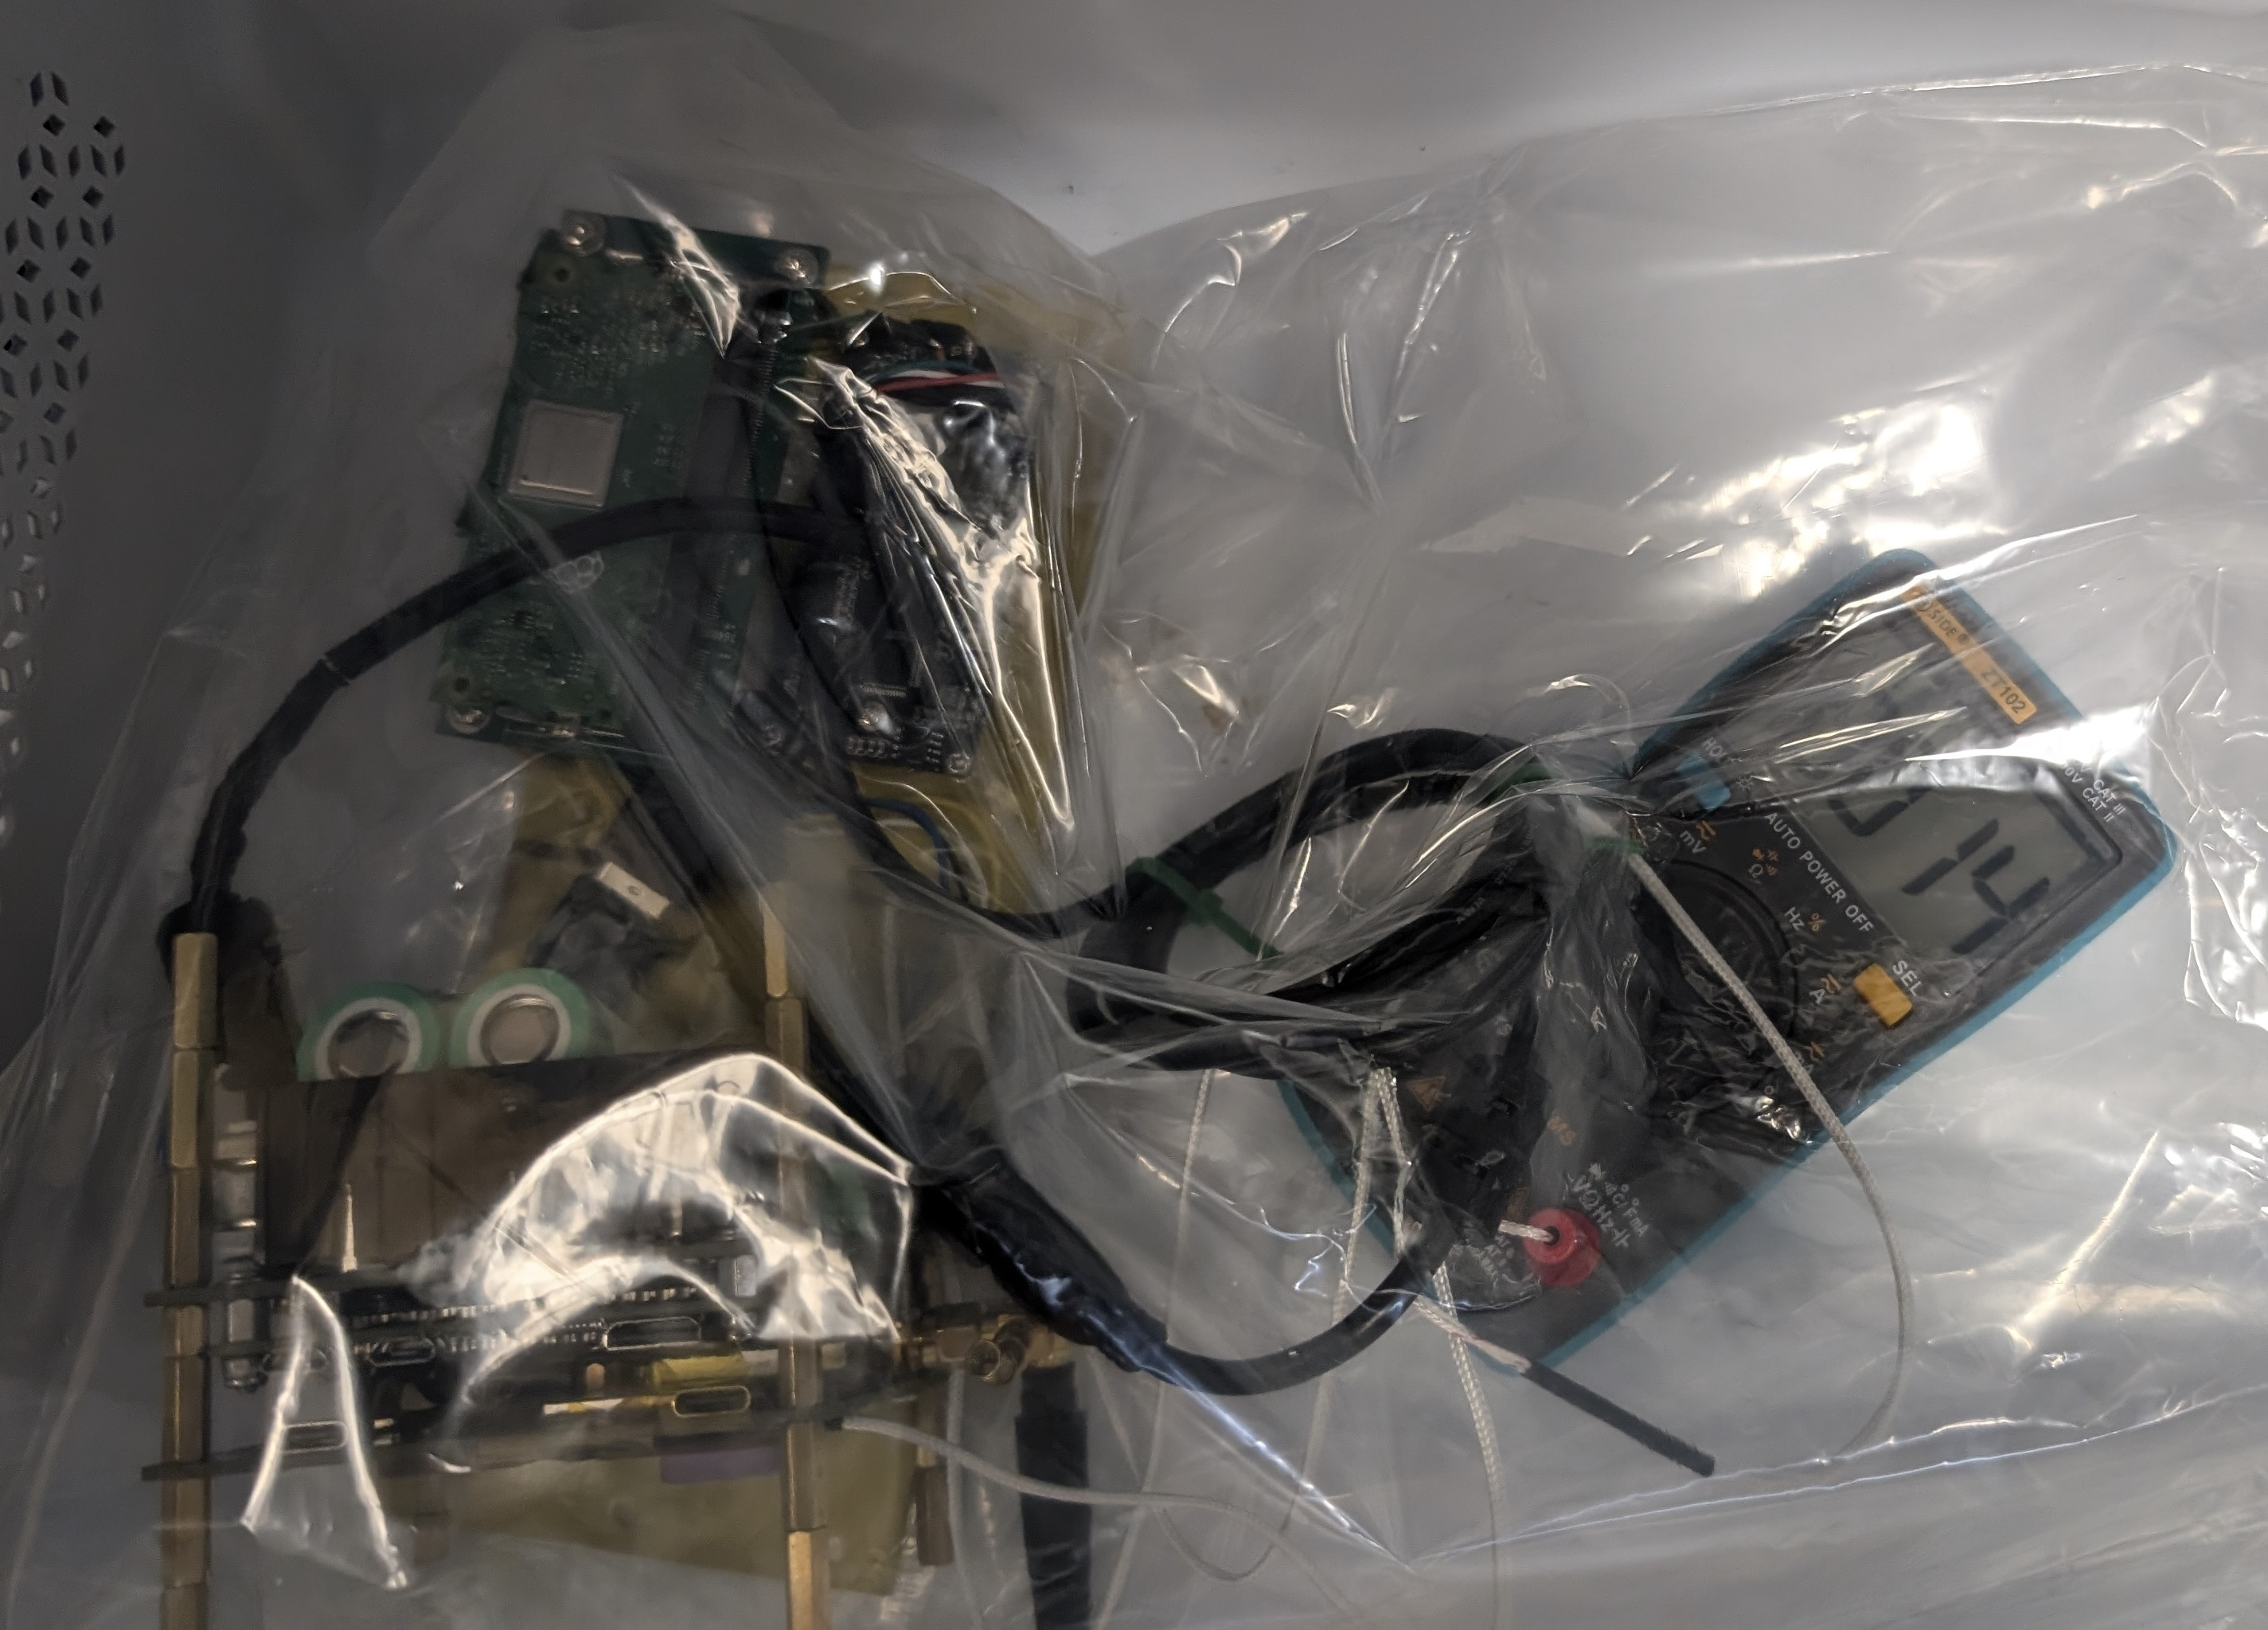
\includegraphics[width=0.75\textwidth]{images/fridge_test.jpg}
  \caption{Low-temperature testing setup}
  \label{fig:temperature-testing-fridge}
\end{figure}

The DAQ was evaluated based on how much time the connection between the DAQ and ground station is lost.

\subsubsection{Shaker table test}  \label{sec:shaker-table-test}

IIST recommends that the CubeSat be mechanically qualified using a single-axis electrodynamic shaker table using random vibration, sine-sweep and half-sine shock tests. 

\paragraph{Random vibration}

The IIST recommended qualification level for the random vibration test is specified in table \ref{tabl:random-vibration-profile-iist}.

\begin{table}[t]
  \centering
  \begin{tabular}{|c | c | c | c | c|}
  \hline
  \textbf{Frequency ($\si{\hertz}$)} & \textbf{PSD ($\si{\square\gacc\per\hertz}$)} & \textbf{$\si{\gacc}$ (RMS)} & \textbf{Duration ($\si{\second\per\siaxis}$)} & \textbf{Axis} \\ \hline
  20  & 0.002 & \multirow{5}{*}{13.5} & \multirow{5}{*}{60} & \multirow{5}{*}{Three axes} \\ \cline{1-2}
  60  & 0.002 &  &  &  \\ \cline{1-2}
  250 & 0.138 &  &  &  \\ \cline{1-2}
  1000 & 0.138 &  &  &  \\ \cline{1-2}
  2000 & 0.034 &  &  &  \\ \hline
  \end{tabular}
  \caption{IIST recommended random vibration test profile for qualification of CubeSat for launch on POEM.}
  \label{tabl:random-vibration-profile-iist}
\end{table}


\begin{figure}[b]
\centering
\includesvg[width=\linewidth]{images/random-qualification-level.svg}
\label{fig:random-vibration-qualification-level}
\caption{IIST recommended random vibration test profile for qualification of CubeSat for launch on POEM (profile defined in \ref{tabl:random-vibration-profile-iist}).}
\end{figure}

This random vibration profile is standard in industry, other launches of satellites on the PSLV use similar vibration profiles.

The IIST recommended random vibration test profile was used without modifications in the final shaker table testing.

% TODO: COMPARE THESE PROFILE TO INDUSTRY STANDARD PROFILES TO BACK THIS UP? SEE EXISTING PAPERS ON PSLV LAUNCH QUALIFICATION
  
\paragraph{Sine-sweep}

The IIST recommended qualification level for the sine-sweep test is specified in table \ref{tabl:sine-sweep-profile-iist}.

\begin{table}[H]
  \centering
  \begin{tabular}{|c|c|c|c|c|c|}
  \hline
  \multicolumn{2}{|c|}{\textbf{Longitudinal}} & \multicolumn{2}{c|}{\textbf{Lateral}} & \multirow{2}{*}{\textbf{Sweep Rate}} & \multirow{2}{*}{\textbf{Axis}} \\ \cline{1-4}
  \textbf{Frequency} & \textbf{Level} & \textbf{Frequency} & \textbf{Level} &  &  \\ \hline
  \SIrange{10}{16}{\hertz} & \SI{20}{\mmDA} & \SIrange{10}{16}{\hertz} & \SI{12}{\mmDA} & \SI{4}{\octave\per\minute} & Three axes \\ \hline
  \SIrange{16}{100}{\hertz} & \SI{10}{\gacc} & \SIrange{16}{100}{\hertz} & \SI{6}{\gacc} & \SI{4}{\octave\per\minute} & Three axes \\ \hline
  \end{tabular}
  \caption{Vibration Data: Longitudinal and Lateral Details with Sweep Rate and Axis Merged}
  \label{tabl:sine-sweep-profile-iist}
\end{table}

\paragraph{Shock}
The IIST recommended qualification level for the shock test is specified in table \ref{tabl:shock-test-iist}.

\begin{table}[H]
\centering
\begin{tabular}{|c|c|c|c|}
\hline
\textbf{Amplitude} & \textbf{Duration (ms)} & \textbf{Shock profile} & \textbf{Axis} \\ \hline
\SI{50}{\gacc} & 10 & Half sine & Single-axis shocks, for all three axes \\ \hline
\end{tabular}
\caption{IIST recommended shock test profile for qualification of CubeSat for launch on POEM.}
\label{tabl:shock-test-iist}
\end{table}



\subsubsection{Drone test flights}

Drone tests were used as a qualification platform for the HPR launch since drone tests:

\begin{enumerate}
  \item Use the expertise of the UWA Aviation Laboratory, which is participating in the project.
  \item Are repeatable, whereas the rocket test can only feasibly be done once per launch season.
  \item Have greater control over the position compared to the suborbital rocket launch and will better qualify the machine vision algorithms.
\end{enumerate}

The drone test evaluates the communications between the camera payload and the communications downlink stability in real time. A successful test involves receiving at least one frame from the camera payload at a reasonable quality.

\subsubsection{High-power rocket test flight}

The high-power rocket (HPR) test flight is used as an experimental qualification method for the CubeSat. This DAQ system is used to evaluate the effectiveness of the HPR flight by using accelerometers, but the HPR flight also serves as a milestone for evaluating the effectiveness of this DAQ for this type of application.

\subsection{Evaluation of accelerometers}

Typical parameters for the evaluation of accelerometers include 

\section{First revision of test and POEM emulation electronics}

The POEM provides services such as tracking, telemetry and command (TT\&C), electrical power system (EPS) and on-board data handling (OBDH) to the CubeSat, therefore these systems are not integrated into the CubeSat under test and must be provided by a separate system on the HPR which emulates the POEM services. The POEM emulator consists of three PCBs: A combined EPS and OBDH board, a tracking board and a telemetry and command board. This emulation and qualification platform will be referred to as DAQ v1.

\subsection{On-board data handling (OBDH)}
Two OBDHs are arranged in a dual redundant configuration and are linked to each other via controller area network (CAN) bus. When the hot spare detects that the primary OBDH is outputting bad data or is not responding, the secondary OBDH will take over control of the communications link. This redundancy ensures the likelihood of not obtaining experiment data for this research is minimised. In the best case, this will provide two independent data sources for research. Both OBDHs will still store data to their respective eMMC modules for post-flight analysis.

\subsection{Accelerometers}
MEMS accelerometers, which will provide the data for this analysis, are located on independent modules and on the OBDH computer. The low-cost LSM6DSO accelerometer will be used due to its low cost and acceleration range of 16-\textit{g} and bandwidth of up to $\SI{6664}{\hertz}$ \cite{lsm6dso-datasheet}, which will be used to cover the quasi-static acceleration and random vibration cases. As shown in figures \ref{fig:random} and \ref{fig:qatforces}, the \textit{g}-levels and bandwidth are relatively low and are met by the LSM6DSO.

The independent accelerometer modules will contain a microcontroller, regulator and accelerometer in a small package which can be mounted at various points on the CubeSat, to measure how evenly the response is applied to the CubeSat. The microcontroller will compress the accelerometer data and send it to the OBDH over CAN bus. The OBDH will generate a clock synchronisation signal to ensure the accelerometer measurements are synchronised. The modules will be attached to the CubeSat using adhesives due to its acceptable performance at the frequencies being measured, and ease of use compared to screws.

Measuring the shock response is significantly more difficult due to the high acceleration levels and the large bandwidth \cite{nasa-pyroshock}, which are not well-suited for low-cost MEMS accelerometers. Instead of measuring the full spectrum, the slope will be measured and compared using the low-cost ADXL373 accelerometer which can measure up to 400-\textit{g} at 2.56 kHz, which is enough to characterise the slope, which is the only parameter required to show that a rocket is inadequate for qualifying shock.

% TODO: shock response

\subsection{Electrical power system (EPS)}
A 2S lithium-ion battery pack and two 5V boost converters will be used to power CubeSat and the emulator. Two independent EPS will be connected in an OR-ing configuration so that if one fails, the other will provide power. The CubeSat and emulator will have separate boost converters, and the power to the CubeSat is capable of delivering the full 5V @ 3A which is the specified amount of power available to the CubeSat on the POEM.

\subsection{Telemetry and command}
An RFD900x radio will be used to downlink the data from the CubeSat and the engineering sensors. This link is optimised for relatively high speed and to have the full 300 kbps capacity that the POEM can provide to the CubeSat. The experiment data required for this research will be downlinked as part of the engineering data, to ensure that data is available to continue research in case the rocket crashes and the onboard memory is destroyed.

The tracking and command system will be on a separate low-bandwidth LoRa radio which is optimised for high link budget and reliability.


\subsection{GNSS Tracking}

The GNSS tracking board contains a standard precision NEO-M9N GNSS receiver and the ZED-F9P differential GNSS (DGNSS) receiver. A NEO-M9N was selected against other standard GNSS receivers due to its high maximum position, velocity and time (PVT) update rate of $\SI{25}{\hertz}$. The main purpose of the NEO-M9N is to serve as a simple backup GNSS receiver for reliable tracking purposes, since it does not require an RTK data stream.

The ZED-F9P differential receiver has centimetre-level accuracy and will enable the heading of the rocket to be accurately determined, which is required for this research since the heading may change throughout the flight and this will need to be accounted for when analysing the data since there are 6 DOF, instead of just one in traditional shaker table tests.

\subsection{Drone testing}
Prior to flight on a HPR the DAQ v1 was tested on a drone. 
TODO:

\begin{itemize}
  \item 
\end{itemize}

\subsection{Results}

One of the objectives of this research is to design a platform for qualification of CubeSats. The first revision of the qualification platform was not used in the final design due to several issues:

\begin{itemize}
  \item The STM32L476 did not have enough resources to move data from the sensors and camera payload to the payload at an adequate speed. A benchmark using CrystalDiskMark, in figure \ref{tabl:daq-v1-diskmark} shows that the maximum throughput is $\SI{0.84}{\mega\byte\per\second}$, and while only 60\% of the throughput is being used as shown in \ref{tabl:daq-v1-sensor-datarate}, between reading from the data sources and writing to the storage there is not enough resources in practice to do this at an adequate speed, resulting in the maximum sampling rate of the sensors to be limited.
  \item Due to space limitations on the rocket, it was not possible to have two redundant systems. The next revision would use only one DAQ.
  \item By the end of this section, it was understood that centimetre level positioning was not required to obtain good results from the camera system.
  \item At the end of this revision it was concluded that the STM32 platform was not flexible enough to complete the research objectives in time.
\end{itemize}

\begin{table}[H]
\centering
\label{tabl:daq-v1-sensor-datarate}
\begin{tabular}{|c|c|p{0.6\linewidth}|}
  Data source & Data rate  & Notes \\ 
  \hline
  LSM6DSOX & $\SI{0.41}{\mega\byte\per\second}$ & $16$ byte structs are generated at $\SI{6664}{\hertz}$ for both acceleration and gyroscope data for two sensors.\\
  ADXL375  & $\SI{0.038}{\mega\byte\per\second}$ & $20$ byte structs generated at $\SI{1}{\kilo\hertz}$ for two sensors.\\
  Camera  & $\SI{0.054}{\mega\byte\per\second}$ & $\SI{460800}{\baud}$ \\
  TOTAL   & $\SI{0.502}{\mega\byte\per\second}$ & $60\%$ of maximum sequential write bandwidth.
\end{tabular}
\caption{Data sources and their data rates.}
\end{table}

\begin{table}[H]
\centering
\begin{tabular}{|c|c|c|}
  Test  & Read [MB/s] & Write [MB/s]\\
  \hline
  SEQ1M Q1T1 (1 task, 1 thread)     & 0.84  & 0.84\\
  % RND4K Q32T1 (32 tasks, 1 thread)  & 0.81  & 0.70\\
  RND4K Q1T1 (1 task, 1 thread)     & 0.75  & 0.66\\
\end{tabular}
\caption{CrystalDiskMark benchmark of DAQ v1.}
\label{tabl:daq-v1-diskmark}
\end{table}

\section{Second revision of test and POEM emulation electronics}
The second revision of the test and POEM emulation electronics (referred to as DAQ v2) contains several improvements and simplifications over DAQ v1.

\subsection{On-board data handling (OBDH)}
A Raspberry Pi Zero W is used for the OBDH system instead of an eMMC module and STM32L476 since:
\begin{itemize}
  \item It reduces the cost of the PCB as the assembly of BGA packages such as eMMC adds significant cost per board,
  \item The Pi Zero W runs an operating system and can be controlled remotely from a PC unlike the STM32, which simplifies development and debugging,
  \item The write speed of the Pi is larger than the STM32 and eMMC combination. % TODO: benchmark write speed.
\end{itemize}

While a Raspberry Pi Zero 2W would be preferable due to its multicore design, due to supply chain issues it was only possible to use a Raspberry Pi Zero W.

DAQ v2 does not have two redundant OBDH due to a lack of room.

\subsection{Accelerometers}

\subsection{Electrical power system (EPS)}

DAQ v2 uses a similar EPS design to DAQ v1, 

\subsection{Telemetry and command}
\subsection{GNSS Tracking}

\section{High-Power Rocket}

A custom rocket named UNO was designed and built by another project member from scratch, it has a height of 290 cm, diameter of $\SI{16.3}{\centi\meter}$ and a dry mass of $\SI{14.42}{\kilo\gram}$ without a motor. It was designed to fly with an M impulse class motor, however due to changes in United States export regulations it was not possible to obtain this motor in the time of this research, and therefore it was only possible to launch with a K impulse class motor which has about 1/10th of the total impulse of the N motor as shown in table \ref{tabl:impulseclasses}.

\begin{table}[H]
\centering
\label{tabl:impulseclasses}
\begin{tabular}{|c|c|}
  Total impulse [$\SI{}{\newton\second}$] & Motor impulse class \\
  \hline
  160.01 - 320.00         & H \\
  320.01 - 640.00         & I \\
  640.01 - 1,280.00       & J \\
  1,280.01 - 2,560.00     & K \\
  2,560.01 - 5,120.00     & L \\
  5,120.01 - 10,240.00    & M \\
  10,240.01 - 20,560.00   & N \\
  20,560.01 - 40,960.00   & O \\
  40,960.01 - 81,920.00   & P \\
  81,920.01 - 163,840.00  & Q \\
\end{tabular}
\caption{Rocket motor impulse classes \cite{nfpa2018}}
\end{table}

\begin{figure}[H]
  \includesvg[width=\textwidth]{images/honors-openrocket2.svg}
  \label{fig:openrocket}
  \caption{OpenRocket diagram of UNO.}
\end{figure}

\subsection{Simulation}

The rocket was simulated using OpenRocket \cite{openrocket,niskanen2009}, an open-source simulator which can predict parameters such as stability and acceleration based on empirical methods which use the rocket's shape and basic environment parameters such as constant wind \cite{doi:10.1177/0954410017752730,niskanen2009}. OpenRocket is used to ensure the rocket design is stable throughout launch and flight, which is important to ensuring the CubeSat payload does not become damaged by this qualification method. However, as it uses a simple empirical model of the flight, it was not designed to model the effect of the motor and aerodynamic forces on the vibration environment in the rocket. It also does not simulate pyroshock events, instead modelling parachute deployment events as simple changes in the aerodynamics of the rocket \cite{niskanen2009}.

\subsubsection{Flight profile}

% TODO: Add motot thrust curve or something with more detial.
As shown in \ref{fig:openrocket-k-launch} the rocket reaches an apogee of \SI{413}{\meter} at \SI{9.74}{\second} and the total flight time is \SI{30}{\second}.

\begin{figure}[H]
  \includesvg[width=\textwidth]{images/k-ork-vertical.svg}
  \label{fig:openrocket-k-launch}
  \caption{Flight profile of UNO using a K1100T motor. Simulated in OpenRocket.}
\end{figure}


\subsubsection{Stability}

As shown in figure \ref{fig:openrocket-k-stability}, the stability is above 2.0 calibres for the coast and launch phase, which is a rule of thumb to ensure the rocket is stable and will not veer off course \cite{canepa2005modern}. The short moment of stability below 2.0 occurs when the rocket reaches apogee, which is not an issue since the parachutes are immediately deployed at this point.

\begin{figure}[H]
  \includesvg[width=\textwidth]{images/k-ork-stability.svg}
  \label{fig:openrocket-k-stability}
  \caption{Stability of UNO using a K1100T motor. Simulated in OpenRocket.}
\end{figure}

\subsubsection{Acceleration}

As stated, since OpenRocket does not model the vibration environment in the rocket and models the rocket as one solid body, only the acceleration of the whole rocket can be modelled. Pyroshock events are not modelled by OpenRocket. The launch phase lasts only \SI{1.6}{\second} and has a high average acceleration of \SI{5.77}{\gacc}, as shown in \ref{fig:openrocket-k-acceleration}. During the coast phase, the rocket is decelerated by gravity as expected and after parachute deployment the rocket only has a small deceleration force.

\begin{figure}[H]
  \includesvg[width=\textwidth]{images/k-ork-acceleration.svg}
  \includesvg[width=\textwidth]{images/k-ork-acceleration-launch.svg}
  \label{fig:openrocket-k-acceleration}
  \caption{Acceleration of UNO using a K1100T motor over (top) the whole flight and (bottom) the thrust phase. Simulated in OpenRocket.}
\end{figure}



\section{Vibration table testing}
% \subsection{UWA vibration table test setup}
\subsection{AVI vibration table test setup}



\section{Rocket test}

% TODO: Put jamir flgiht data here.

\section{Drone tests}
\subsection{First test}
\subsection{Second test}


\section{Data collection and analysis}

The system will be used for the vibration tests on a shaker table, and the rocket test. The data will be recorded as a time series on the OBDH memory. The time series data will be transformed into the frequency domain since existing studies have presented frequency domain plots to present and analyse the response of the system to a test \cite{nasa-pyroshock,nieto2019cubesat}. For the rocket test, the analysis will be split over the several phases of flight - launch, thrust, coast and parachute deployment events, since the forces involved are different in all of these phases.

\subsection{Shock}
\subsubsection{Vibration table results}
\subsubsection{HPR results}
\subsubsection{Comparison of methods}
In the launch and parachute deployments, where pyrotechnics are ignited, an analysis of the shock response spectrum will be performed. This will involve creating the shock response spectrum for the rocket test and shaker table tests, then comparing the slope up to ~1 kHz. If the rocket test SRS slope is on the same order of magnitude as the gradient found in \cite{wang2023numerical} for other low explosives, and it is less than the slope of the SRS from the shaker table tests, then this will show that rocket testing is not an adequate qualification method for shock.

\subsection{Random}
\subsubsection{Vibration table results}
\subsubsection{HPR results}
\subsubsection{Comparison of methods}
The coast phase, where the rocket motor has burnt out but is still approaching apogee, will be compared to the random vibration test. The random response spectrum will be compared to the spectrum of the rocket test to check how uniformly distributed the rocket test is.

\subsection{Quasi-static acceleration}
\subsubsection{Vibration table results}
\subsubsection{HPR results}
\subsubsection{Comparison of methods}
The boost phase will be compared to the quasi-static acceleration tests on the shaker table. It is expected that the acceleration force on the HPR will be greater than those experienced on the launch vehicle, however the key characteristic - a peak in acceleration over a narrow frequency band - should be the same.

\section{Conclusion}
\subsection{Future work}

Hardware changes for a future revision of the data acquisition system include:

\begin{itemize}
  \item Use Raspberry Pi Zero 2W instead of Zero W since it has more cores.
\end{itemize}

\section{References}

\printbibliography[heading=none]

\section{Appendix}



\end{document}
